\documentclass[]{final_report}
\usepackage{graphicx}
\usepackage{hyperref}
\usepackage{sectsty}
\usepackage{subcaption}
\usepackage{listings}


%%%%%%%%%%%%%%%%%%%%%%
%%% Input project details
\def\studentname{Vinay Kakkar}
\def\reportyear{2023}
\def\projecttitle{Structural Bioinformatics Framework using a MapReduce formalism}
\def\supervisorname{Hugh P. Shanahan}
\def\degree{MSc in Computer Science}
\def\fullOrHalfUnit{Full Unit} % indicate if you are doing the project as a Full Unit or Half Unit
\def\finalOrInterim{Final Report} % indicate if this document is your Final Report or Interim Report
\sectionfont{\clearpage}
\begin{document}

\maketitle

\newtheorem{definition}{Definition}[section]
\renewcommand\thesection{\arabic{section}}

\begin{abstract}
    Need a abstract
\end{abstract}

\section{Rationale: 10 marks}
\subsection{Aims}
\subsubsection{Aim provided in the Project Description}
"The aim of this project is to be provide a framework where large numbers of protein structures can be analysed using a user-provided executable in the MapReduce formalism."

\subsubsection{Aim}
Analysing protein structures can provide insights into their properties and interactions with other molecules. However, analysing large numbers of protein structures can be computationally intensive, requiring significant computational resources and time. Thus, the aim is to provide a framework that allows for the analysis of large numbers of protein structures using a MapReduce formalism.

\textbf{\textit{MapReduce:}} is a programming model for processing and generating large data sets. Allowing for parallel processing of data across multiple nodes in a cluster, making it well-suited for analysing large datasets.

More specifically the aim is to develop a framework that can take a user-provided executable and apply it to a large number of protein structures in a parallel, distributed manner using MapReduce. This will enable researchers to perform complex analyses on large datasets of protein structures more efficiently, saving time and computational resources. Essentially enabling researchers to analyse large numbers of protein structures more quickly and effectively than before.\\
\clearpage
\subsection{Objectives}

To achieve the aim of the project, the following objectives have been formulated:

\begin{itemize}
    \item Develop a software framework that suppots the Mapreduce formalism and can process large numbers of protein structures.
    \item Implement a distributed computing system using MapReduce to parallelize protein structure analysis across multiple computing nodes.
    \item Optimize the software framework to reduce the processing time required for protein structure analysis.
    \item Validate the software framework by testing it with a variety of protein structure analysis tools and evaluating its performance in comparison to other available tools.
\end{itemize}
The software must provide the ability to perform quicker and efficiently by allowing executables to be perfomred on multple files in a parallel compared to current solutions.\\\\

\begin{itemize}
    \item Design an interface that allows users to manipulate the pdbs that are being passed into the executable for protein structure analysis.
\end{itemize}
The software revolves around using and manipulatting PDB files so the framework should give the user a method/function which is able to search and input pdb files automatically\\\\

\begin{itemize}
    \item Ensure the software framework is scalable and can handle increasingly large datasets.
    \item Ensure the software framework can be eaisly updated to keep pace with advancements in protein structure analysis techniques and computing technology.
\end{itemize}
The pdb database is changing frequently with more protein structres being added exponetialy. The software should be able to cope with changes and by working with the fundamental set out standerds set out for uploaded protien structures.\\\\

\begin{itemize}
    \item Provide documentation and user support to enable researchers to use the software framework effectively.
\end{itemize}
The framework should contain multiple functions that the user can use in order to perform executables on a set number of pdb files and query the pdb database in order to set up the files required by the user.\\\\

\subsubsection{Software Framework and MapReduce}
The software framework must support a Mapreduce formalism that can process large numbers of protein structures. Where the MapReduce formalism consists of two main functions: Map and Reduce. The Map function takes a set of data and transforms it into another set of data, where individual elements are broken down into key-value pairs. The Reduce function then takes the output of the Map function and combines all the values associated with a given key, producing a final output for each key. More specifically each map and reduce step can be conducted through multiple nodes.


\subsubsection{Interface and Documentation}
\subsubsection{Further Objectives}


\subsection{Introduction}
Structural bioinformatics plays a critical role in the development of new drugs, as well as in understanding the molecular basis of biological processes. It involves the analysis and interpretation of large amounts of complex data, including the three-dimensional structures of proteins, DNA, and other macromolecules. As the size and complexity of these data sets continue to increase, the need for efficient and scalable computational tools for their analysis and processing becomes ever more pressing.

One promising approach to addressing this challenge is the use of MapReduce, a programming model for large-scale data processing in distributed computing environments. MapReduce enables the parallel processing of large data sets across multiple nodes in a cluster, which can significantly improve the speed and efficiency of data analysis tasks.

In this report, we present a structural bioinformatics framework that utilizes a MapReduce formalism for the efficient analysis of large-scale structural data. Our framework is based on a distributed computing architecture that allows for the parallel processing of structural data, including protein structures, protein-protein interactions, and other molecular structures. We describe the key components of our framework, including the data preprocessing, map, and reduce phases, as well as the parallel algorithms and data structures used to implement these phases.

We demonstrate the effectiveness of our framework through a series of experiments on real-world structural data sets, showing that our approach can significantly reduce the time and resources required for complex bioinformatics tasks. Our results highlight the potential of MapReduce-based approaches for accelerating the analysis of large-scale structural data in the field of bioinformatics.





\section{Literature Review and Background Reading: 15 marks}
\subsection{Protein Structures}
\subsubsection{Introduction}

Amino acids are molecules that when combined forms proteins. All of the 20 amino acids, see table~\ref{Amino acids} have in common a central carbon atom which is attached to a hydrogen atom, an amino group, and a carboxyl group~\cite{branden_introduction_1998}.

Proteins are responsible for catalysing most of the chemical reactions in cells. They can function as enzymes catalysing a wide variety of reactions important for life and thus also important for the structure of living systems such as proteins involved in the cytoskeleton. The size of protein can vary ~\cite{zvelebil_understanding_2008}.

\begin{definition}[Catalysing]
    Catalysing is to make a chemical reaction happen or happen more quickly by acting as a catalyst.
\end{definition}

\begin{definition}[Cytoskeleton]
    A dynamic network of interlinking protein filaments present in the cytoplasm of all cells~\cite{zvelebil_understanding_2008}. 
\end{definition}

\subsubsection{Primary, Secondary, Tertiary and Quaternary Structure}

Please refer to~\ref{fig:levels of protein structure.} for a visual representation.

The \textbf{primary structure} of a peptide or protein is the linear sequence of its amino acids. It is read and written from the amino-terminal to the carboxyl-terminal end.~\cite{sun_overview_2004}.

The \textbf{secondary structure} refers to the local arrangement of a peptide chain. Where several common secondary structures have been identified in proteins~\cite{sun_overview_2004}.

\textbf{Tertiary structure} is a three-dimensional structure of a protein the formation is built up of bonds and interactions that serve to change the shape of the overall protein~\cite{godbey_chapter_2022}.

The \textbf{quaternary structure} of a protein is built-up of several protein chains/subunits. Each of the subunits has its primary, secondary, and tertiary structure~\cite{ouellette_14_2015}.

\begin{table}[h!]
    \begin{center}\label{tab:Amino acids}
        \begin{tabular}{l|c|r}
        Amino acid & Three-letter code & One-letter code\\
        \hline
        \\
        Glycine & Gly & G\\
        Alanine & Ala & A\\
        Valine & Val & V\\
        Leucine & Leu & L\\
        Isoleucine & Ile & I\\
        Proline & Pro & P\\
        Phenylalanine & Phe & F\\
        Methionine & Met & M\\
        Tryptophan & Trp & W\\
        Cysteine & Cys & C\\
        \\
        \hline
        \\
        Asparagine & Asn & N\\
        Glutamine & Gln & Q\\
        Serine & Ser & S\\
        Threonine & Thr & T\\
        Tyrosine & Tyr & Y\\
        \\
        \hline
        \\
        Aspartic acid & Asp & D\\
        Glutamic acid & Glu & E\\
        \\
        \hline
        \\
        Histidine & His & H\\
        Lysine & Lys & K\\
        Arginine & Arg & R\\
        \end{tabular}
        \caption{\label{Amino acids}The 20 amino acids. The amino acid name, the three-letter code, and the one-letter code are given. The Amino acids are split up into Nonpolar, Polar, Acidic and Basic respectfully}
    \end{center}
\end{table}

\begin{figure}[h]
    \centering
    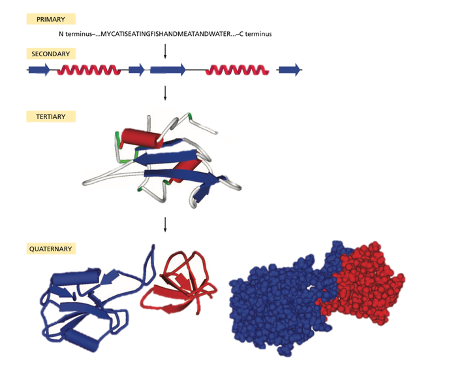
\includegraphics[width=0.5\textwidth]{Protein Structure.png}
    \caption{\label{fig:levels of protein structure.}From the sequence alone, the primary structure to secondary structure, to tertiary structure(3D), to finally quaternary structure found when several tertiary structures form a multisubunit complex~\cite{zvelebil_understanding_2008}.}
\end{figure}

\subsubsection{Considering Protein structure on several different levels}

The fold of the protein plays part in determining the way the protein will function, and also whether it will function correctly. As there are Protein structures on different levels we need to consider the analysis of protein structure by experimental techniques such as X-ray crystallography, nuclear magnetic resonance, and RNAseq which show that proteins adopt distinct structural elements~\cite{zvelebil_understanding_2008}.

\subsubsection{Amino Acids}

Sequence of amino acids~\ref{Amino acids} will build up the linear protein chain~\cite{zvelebil_understanding_2008}. Amino acids are different from each other due to their side chains and due to this the functional properties of various different proteins are different~\cite{zvelebil_understanding_2008}. You can see the amino acids grouped here~\ref{Amino acids}.

\subsection{Large Scale Experssion}

Gene expression begins when genes are transcribed into messenger RNAs, which are then translated to produce proteins. 

Total gene expression in cultured cells or a tissue sample can be detected in three main ways:

\begin{enumerate}
    \item DNA microarray technology.
    \item Two-dimensional Gel electrophoresis or Chromatography.
    \item RNAseq
\end{enumerate}

Both DNA microarray technology and Two-dimensional Gel electrophoresis, produce enormous amounts of raw data~\cite{zvelebil_understanding_2008} due to this, many proteins currently evade high-resolution structure determination.

\subsubsection{Structural mass spectrometry}
Structural mass spectrometry is a powerful approach used to determine the 3D structure of biological protiens it has nearly an unlimited size constraint and speed. Although the data provided by mass spectrometry is vague for full high-resolution structure elucidation, structural mass spectrometry can be used to examine the size, solvent accessibility, and topography of proteins~\cite{limpikirati_covalent_2018}~\cite{liu_mass_2020}.

We can have computational methods that aid experimental technique intending to elucidate protein structures~\cite{seffernick_hybrid_2020}~\cite{leman_macromolecular_2020}. Software packages can be used to combine data with advanced structure sampling and scoring techniques. Computational tools for protein structure modeling, include the Rosetta software suite~\cite{leman_macromolecular_2020}~\cite{alford_rosetta_2017}, I-TASSER~\cite{yang_i-tasser_2015}, Phyre2~\cite{kelley_phyre2_2015}, Integrative Modeling Platform~\cite{russel_putting_2012}, HADDOCK~\cite{dominguez_haddock_2003}, and MODELLER~\cite{eswar_comparative_2006}~\cite{biehn_protein_2022}.

\subsubsection{Large Scale Gene Expression}

Genome DNA microarray experiments produce large amount of data can be computationaly heavy on where methods can yield alternative conclusions from inceasing the computational effort.

The goal of these experiments is to determine biological or functional meaning from the lists of genes, either by:

\begin{enumerate}
    \item Identify critical genes that are responsible for a biological effect.
    \item Find patterns within the genes that point to an underlying biological process.
\end{enumerate}
\cite{zvelebil_understanding_2008}

\begin{figure}[ht]
    \centering
    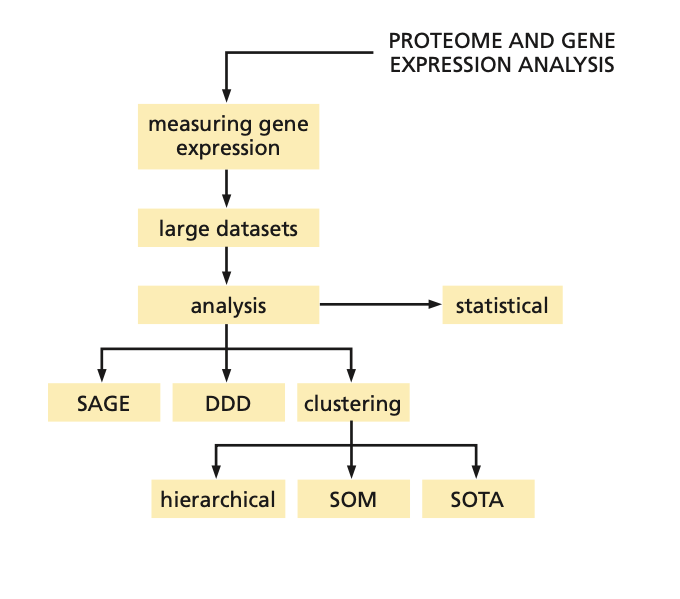
\includegraphics[width=0.5\textwidth]{Gene Expresion.png}
    \caption{\label{fig:Gene Expression}Describing Common experimental aspects of gene expression and of the analysis of the resulting data~\cite{zvelebil_understanding_2008}.}
\end{figure}

\subsubsection{Serial analysis of gene expression}

Serial analysis of gene expression is the alternative compared to microarrays when trying to investigate patterns of gene expression.

\begin{figure}[!h]
    \centering
    \begin{subfigure}[t]{.45\textwidth}
        \centering
        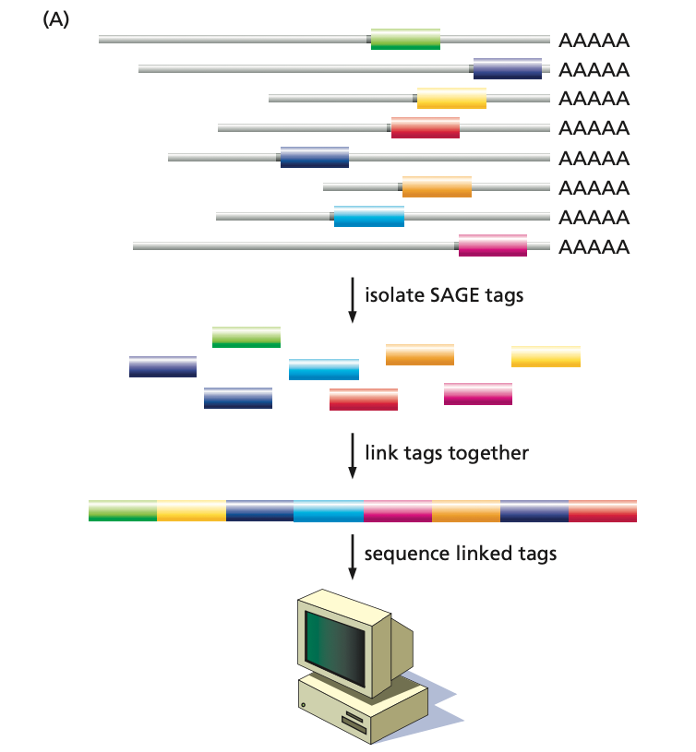
\includegraphics[width=0.9\textwidth]{SAGE1.png}
        \caption{}
        \label{fig:SAGE1} 
    \end{subfigure}
    \begin{subfigure}[t]{.45\textwidth}
       \centering
       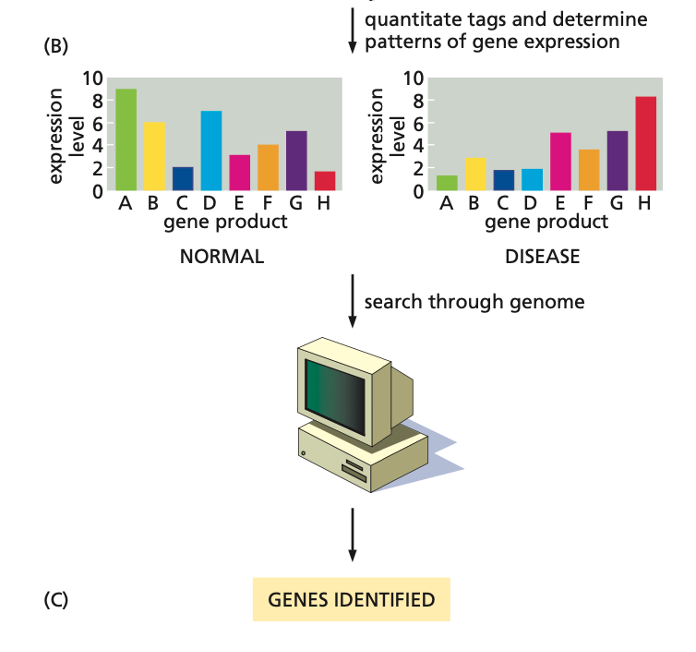
\includegraphics[width=0.9\textwidth]{SAGE2.png}
       \caption{}
       \label{fig:SAGE2}
    \end{subfigure}
    \caption{\emph{An outline of the SAGE method for comparing levels of gene expression. (A) Short sequence tags. The sequence tags are isolated and are linked together to produce long DNA molecules that can be cloned and sequenced. (B) Once sequenced, each tag can be calculated, resulting in a value that gives the expression level of the corresponding transcript~\cite{zvelebil_understanding_2008}.}}\label{fig:SAGE}
\end{figure}

A short sequence contains enough information to uniquely identify a gene. The sequence tags from the total cellular RNA can be linked together to form long DNA molecules. The total number of times a particular tag is observed the concatemers approximates the expression level of the corresponding gene. The data produced by SAGE include a list of the tags with their corresponding counts, providing a digital output of cellular gene expression.  Which allows the user to specify which organ is to be investigated. Libraries consisting of gene lists organized by the various types of tissues or cell lines are provided for further choice. The output from SAGE provides the SAGE tag, the UniGene ID, the gene description, and color and letter-coded differences in expression levels~\cite{zvelebil_understanding_2008}.

\subsubsection{Clustered gene expression data}

Clustered pattern data obtained from gene expression microarrays/genome bioinformatics can be used as a tool to identify new transcription factors or other cell-regulatory proteins. 

The clustered genes/proteins can be analyzed. Leading to a vast collection of data from many gene/protein expression experiments being available on the Web~\cite{zvelebil_understanding_2008}.

\subsubsection{Large Scale Protein Expression}

\begin{figure}[ht]
    \centering
    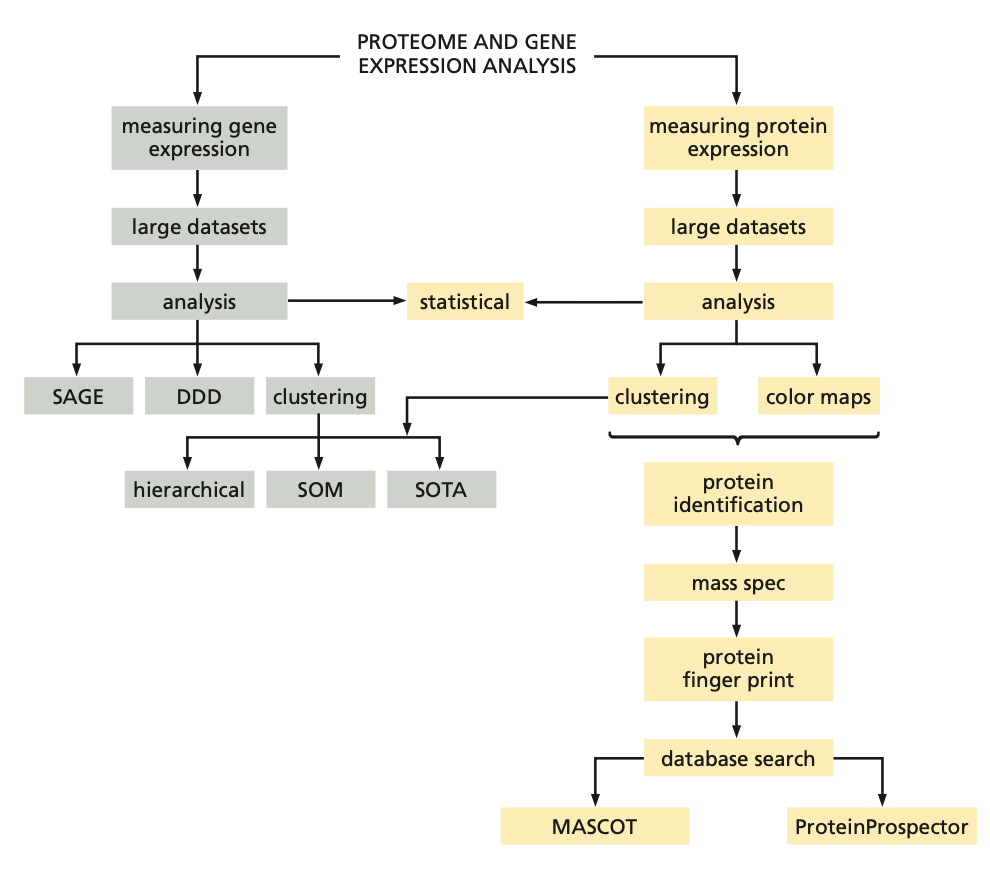
\includegraphics[width=0.5\textwidth]{Overlaping.png}
    \caption{\label{fig:Overlaping}Describing some experimental aspects of protein expression and of the analysis of the resulting data.~\cite{zvelebil_understanding_2008}.}
\end{figure}

For functional protein, mRNAs need to be translated, whilst the protein products can change which influence their function. For this reason we can measure and anlayse different proteins. 

There is more proteins than there are genes in a genome. Transcripts can be spliced in various ways to give different mRNAs, providing different protein products, from the same gene. However, proteins that can be modified after translation giving more different protien products.

Protien expressions can vary in a organism depending on the origin and it will also differ between the separate stages of an organism’s life cycle and under different environmental conditions~\cite{zvelebil_understanding_2008}.

\begin{definition}[proteome]
    The proteome refers to all the proteins that make up an organism at a specific point in time and under specific conditions.
\end{definition}

\subsubsection{RNAseq}

The transcriptome is important for revealing the molecular constituents of cells and tissues, interpreting the functional aspects of the genome, also for understanding development and disease~\cite{wang_rna-seq_2009}.

Many methods deduce and quantify the transcriptome, including hybridization or sequence-based approaches. For example, hybridization-based approaches involve incubating fluorescently labeled cDNA with microarrays or commercial high-density oligo microarrays~\cite{wang_rna-seq_2009}.

However, these methods have several limitations, such as: 
\begin{itemize}
    \item Dreliance upon existing knowledge about genome sequence.
    \item Limited dynamic range of detection owing to both background.
    \item High background levels owing to cross-hybridization~\cite{okoniewski_hybridization_2006}~\cite{royce_toward_2007}.
    \item saturation of signals.
\end{itemize}

\begin{definition}[transcriptome]
    The transcriptome is the complete set of transcripts in a cell, and their quantity, for a specific developmental stage or physiological condition. 
\end{definition}

Sequence-based approaches directly determine the cDNA sequence such as Tag-based methods which include SAGE, CAGE~\cite{kodzius_cage_2006}, MPSS~\cite{reinartz_massively_2002}.

Each approach is high throughput and can provide precise, gene expression levels. However, a significant portion of the short tags can not be uniquely mapped to the reference genome~\cite{wang_rna-seq_2009}.

RNA-Seq RNA sequencing has clear advantages over existing approaches it uses deep sequencing technologies where a population of RNA is converted to a library of cDNA fragments with adaptors attached to one or both ends. Each molecule is then sequenced in a high-throughput manner to obtain short sequences from one or both ends~\cite{wang_rna-seq_2009}.

\begin{figure}[ht]
    \centering
    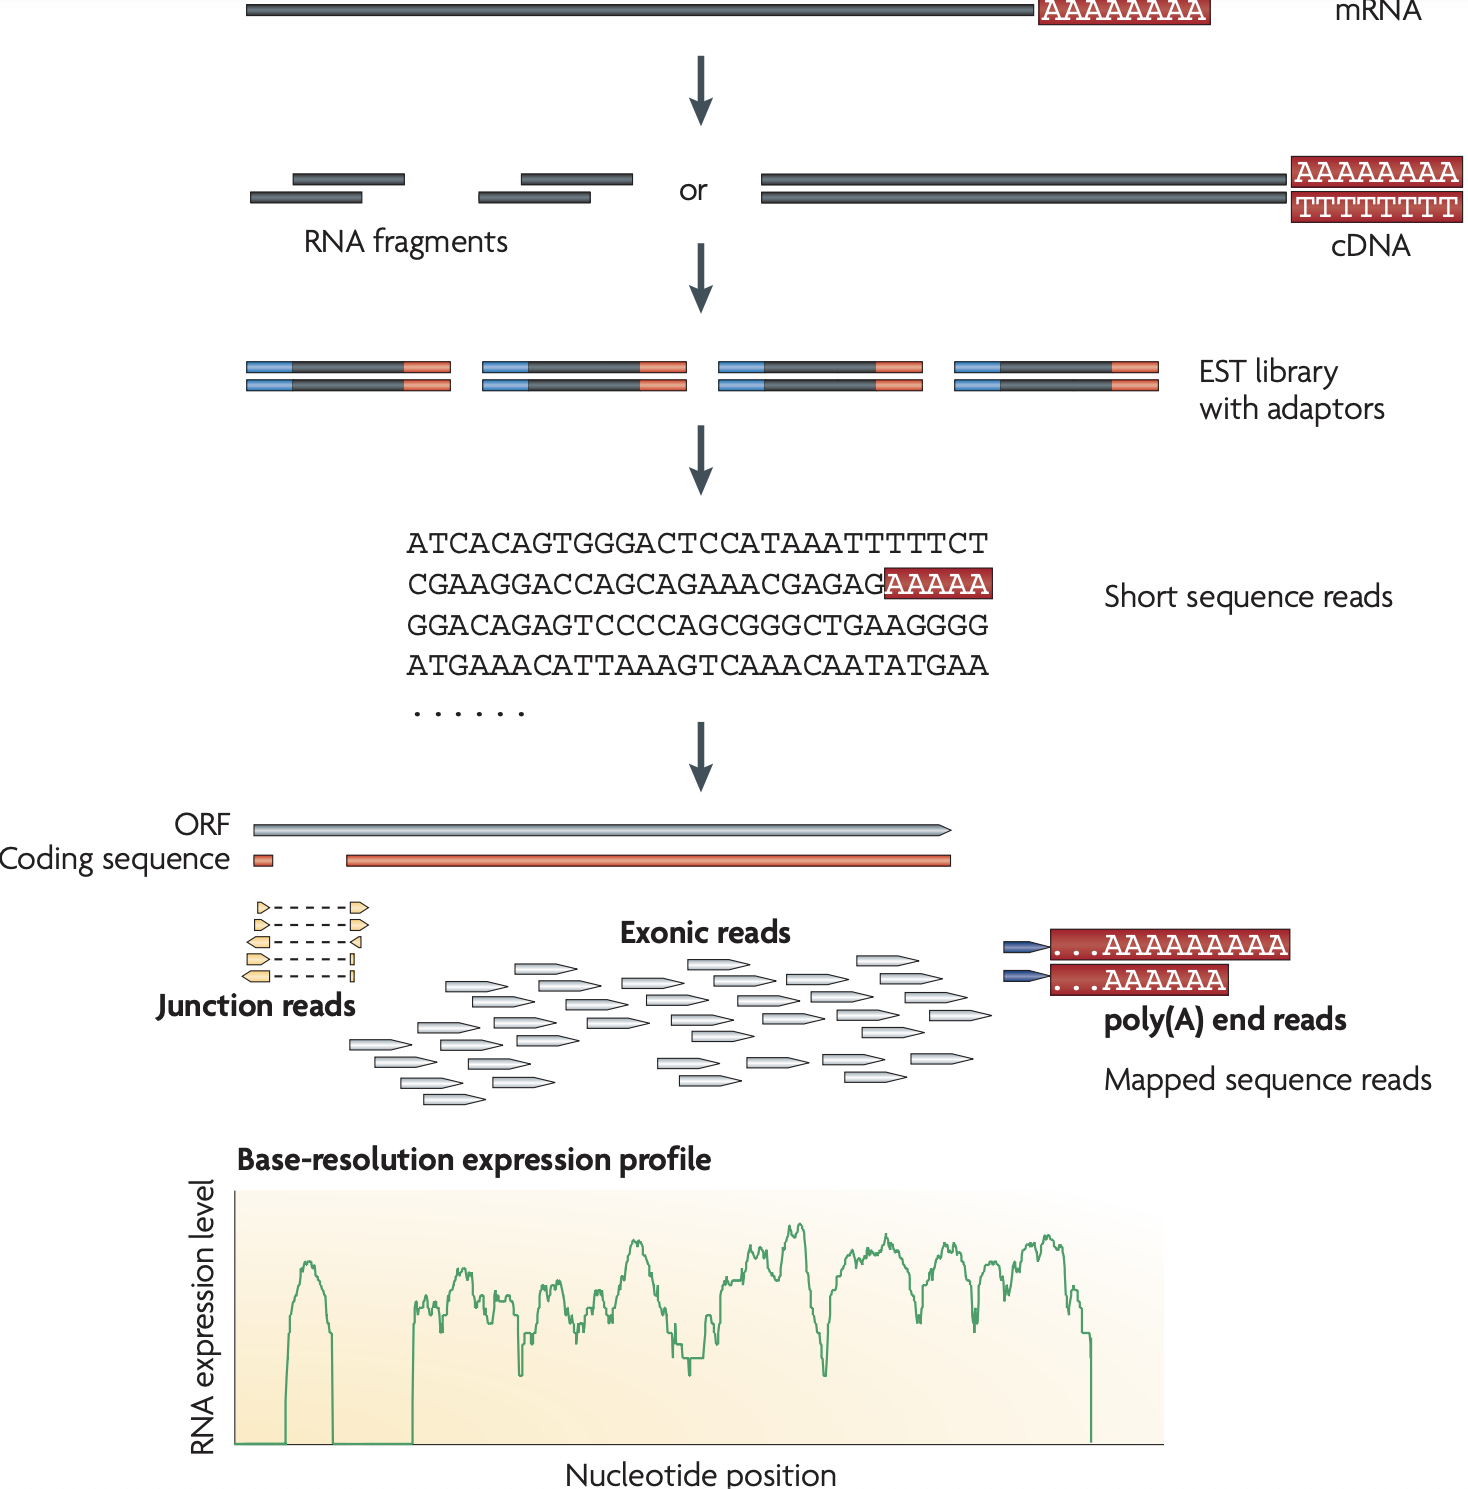
\includegraphics[width=0.5\textwidth]{RNAseq.png}
    \caption{\label{fig:RNAseq}A typical RnA-seq experiment. RNAs are first converted into a library of cDNA fragments through either RNA fragmentation or DNA fragmentation. Sequencing adaptors are subsequently added to each cDNA fragment and a short sequence is obtained from each cDNA using high-throughput sequencing technology. The resulting sequence reads are aligned with the reference genome or transcriptome.}
\end{figure}

\subsubsection{Bioinformatic Difficulties with Predictions on Proteins}

It is difficult to define the precise ends of the helices(The secondary structure of proteins is made up of a-helices and b-strands) for structures found in globular proteins that are not perfectly regular. Making it one step more difficult when trying to predict these structures~\cite{zvelebil_understanding_2008}.

To Note:
\begin{itemize}
    \item Several different types of b-sheet are found in protein structures.
    \item Turns, hairpins, and loops connect helices and strands. 
    \item Any chain between two regular structures is referred to as a loop.
    \item Mostly a loop will contain a turn (or even several).
\end{itemize} 

In antibody recognition, immunoglobulins employ loops at the edge of a b-sheet. All immunoglobulin structures with the same overall chain fold, but it is the difference at these loops that results in different results. Loops take up one of a limited number of structures called canonical forms. This type of classification is another reason why trying to predict both the structure and function of the protein is difficult~\cite{zvelebil_understanding_2008}.

\begin{definition}[Immunoglobulin]
    Immunoglobulins are heterodimeric proteins composed of two heavy and two light chains. Types of white blood cells that helps the body fight infection~\cite{schroeder_structure_2010}.
\end{definition}

\textbf{\textit{NOTE: Need to read and re write and move to before we talk about alphafold}}

\subsubsection{Alpha Fold}

AlphaFolds' goal is to predict the 3D coordinates of all heavy atoms for a given protein using the primary amino acid sequence and aligned sequences of homologues as inputs~\cite{jumper_highly_2021}.

Mutations in proteins can lead to misfolding which is often associated with disease states, for example, Alzheimer’s and Parkinson’s which is one of the challenges for alphaFold~\cite{felix_brief_nodate}.

The output is a file containing the 3D coordinates for every non-hydrogen atom in the protein. whilst showing the confidence levels for every amino acid residue, providing the reliability of the predicted structure~\cite{felix_brief_nodate}.

\subsubsection{Bioinformatics with Alpha Fold}

In July 2021, AlphaFold was developed by DeepMind and was made available to
the public~\cite{tunyasuvunakool_highly_2021}. 

Where it tries to solve the issue of invariant protein structures that are under translations and rotations~\cite{baldi_principled_nodate}.

AlphaFold is trained on protein chains from the PDB using the input sequence to query databases of protein sequences to generate a multiple sequence alignment~\cite{jumper_highly_2021}. Although we still do not exactly know how a protein sequence folds and alpha fold do not help in figuring this out its impact will likely be in accelerating and improving the production of new medications~\cite{nussinov_alphafold_2022}.


\subsubsection{AlphaFold 2}

The CASP14 was recently held which is a blind trial that critically assesses
techniques for protein structure prediction~\cite{david_alphafold_2022}, AlphaFold2 was entered and out-performed all competitors. 

Recently, RoseTTAFold was developed, trying to implement similar principles. Since then, other end-to-end structure predictors have emerged using different principles such as fast multiple sequence alignment processing in DMPFold218 and language model representations.\cite{bryant_improved_2022}.

We use the root mean square deviation, to calculate the similarity between the two structures, AlphaFold models had an accuracy of 0.96 compared to 2.80 which was the second-best score. AlphaFold models also had a high level of accuracy in predicting the position of residue side chains when the protein backbone prediction was accurate~\cite{david_alphafold_2022}~\cite{jumper_highly_2021}.

\subsection{The Protein Data Bank and the File Formats}

\subsubsection{Protein Data Bank}

The Protein Data Bank was established at Brookhaven National Laboratories ~\cite{bernstein_protein_1977} in 1971 as an archive for biological macromolecular crystal structures~\cite{berman_protein_2000}.

\begin{definition}[Macromolecular]
    Macromolecular is any very large molecule, usually with a diameter ranging from about 100 to 10,000 angstroms
\end{definition}

It is an information source for data retrieved from atomic structures, crystallography, and three-dimensional structures of biomolecules, including nucleic acids and proteins~\cite{behzadi_worldwide_2021}. 

At the time this was the first open-access digital data resource in biology which started with just seven protein structures~\cite{burley_rcsb_2022}.

Various groups such as the Protein Data Bank in Europe, Protein Data Bank Japan help manage the Protein Data Bank archive. Current wwPDB members also include the ElectronMicroscopy Data Bank and the Biological Magnetic Resonance Bank~\cite{burley_rcsb_2022}.

Protein Data Bank China has recently joined the wwPDB as an Associate Member with its role as wwPDBdesignated PDB Archive Keeper. Where they are responsible for weekly updates of the archive and safeguarding both digital information and a physical archive of correspondence~\cite{burley1_rcsb_2022}.

The management of PDB must comply with FAIR (the acronym depicts: Findable, Accessible, Interoperable, Reusable) and FACT~\cite{van_der_aalst_responsible_2017} guiding principles for scientific data~\cite{wilkinson_fair_2016}~\cite{westbrook_impact_2020}.

\begin{table}[h!]
    \begin{center}
    \label{tab:FAIR}
        \begin{tabular}{c|p{0.65\linewidth}}
        The FAIR Guiding Principles\\
        \hline
        \\
        To be Findable: & F1. (meta)data are assigned a globally unique and persistent identifier\\
        & F2. data are described with rich metadata (defined by R1 below)\\ & F3. metadata clearly and explicitly include the identifier of the data it describes\\ & F4. (meta)data are registered or indexed in a searchable resource\\
        \\
        \hline
        \\
        To be Accessible: & A1. (meta)data are retrievable by their identifier using a standardized communications protoco\\
        & A1.1 the protocol is open, free, and universally implementable\\ & A1.2 the protocol allows for an authentication and authorization procedure, where necessary\\ & A2. metadata are accessible, even when the data are no longer available
        \\
        \hline
        \\
        To be Interoperable: & I1. (meta)data use a formal, accessible, shared, and broadly applicable language for knowledge representation.\\
        & I2. (meta)data use vocabularies that follow FAIR principles\\ & I3. (meta)data include qualified references to other (meta)data\\
        \\
        \hline
        \\
        To be Reusable: & R1. meta(data) are richly described with a plurality of accurate and relevant attributes\\
        & R1.1. (meta)data are released with a clear and accessible data usage license\\ & R1.2. (meta)data are associated with detailed provenance\\ &
        R1.3. (meta)data meet domain-relevant community standards\\
        \end{tabular}
        \caption{\label{Fair}The guidlines to what builds up the FAIR principles~\cite{wilkinson_fair_2016}}
    \end{center}
\end{table}

\subsubsection{Aims and Objectives of PDB}

Enzymology, electron microscopy, computational chemistry small molecule crystallography, biochemistry, biophysics, macromolecular crystallography and nuclear magnetic resonance spectrometry all help the aims and goals of the PDB archive~\cite{behzadi_worldwide_2021}.

\begin{definition}[Enzymology]
    Enzymology is the branch of biochemistry aiming to understand how enzymes work
\end{definition}

\begin{definition}[Electron Microscopy]
    Electron microscopy is a technique for obtaining high resolution images of biological and non-biological specimens.
\end{definition}

PDBs provide open access to nearly 200 000 archived, validated, and biocurated experimentally determined three-dimensional structures of biological macromolecules.3D structures archived in the PDB have enabled important scientific breakthroughs by basic and applied researchers~\cite{burley_impact_2021}. Open access to PDB data without restrictions on usage has also aided structural bioinformatics in areas such as computational biology.

\subsubsection{Recent Project}

A project was undertaken to change the information management services for RCSB.org. The idea was to have developed a primary place for studying 3D biostructures by extending RCSB.org web portal functionality to support parallel delivery of more than one million CSMs publicly available from AlphaFold DB and ModelArchive together~\cite{burley1_rcsb_2022}.

\subsubsection{Covid}

During the COVID-19 pandemic, more than 2000 structures associated with the agent of the coronavirus disease were released and have become accessible to global users for free. The properties of these structures give us this opportunity to find out the ligand binding sites, the spatial conformation of ligands, protein-to-protein interactions, and amino acid substitutions regarding different viral proteins. Moreover, chemical, functional and energetic characteristics can also be gained to describe the potential capabilities of each molecule. These properties might aid us to determine the potential drug targets for drug design and vaccine preparation~\cite{lubin_evolution_2020}.

\subsubsection{PDB Currently}

As of 2022, the PDB has a vast number of 3D biostructures, eukaryotic protein structures exceeded 105 000. Bacterial protein structures were also numerous, totaling nearly 66 000. Archaeal protein structures were the least numerous totaling 5500. However the PDB coverage is decidedly limited, with mouse protein structures being most numerous at 8000 structures~\cite{burley_open-access_2021}. 

We have powerful tools developed by RCSB PDB for searching and analysis which include structure, sequence, sequence motif, structure motif, and visualization~\cite{burley1_rcsb_2022}.

Upon reaching the RCSB.org home page, users can query, organize, visualize, analyse, compare, and explore PDB structures and CSMs side-by-side. Searching 3D structure information can encompass PDB structures and CSMs or be limited to PDB structures only. Either PDB structures or CSMs can be excluded from the search results. The two types of structure information accessible via RCSB.org are clearly distinguished from each other. Top bar searching and data delivery for PDB structures and CSMs~\cite{burley1_rcsb_2022}.

\begin{figure}[ht]
    \centering
    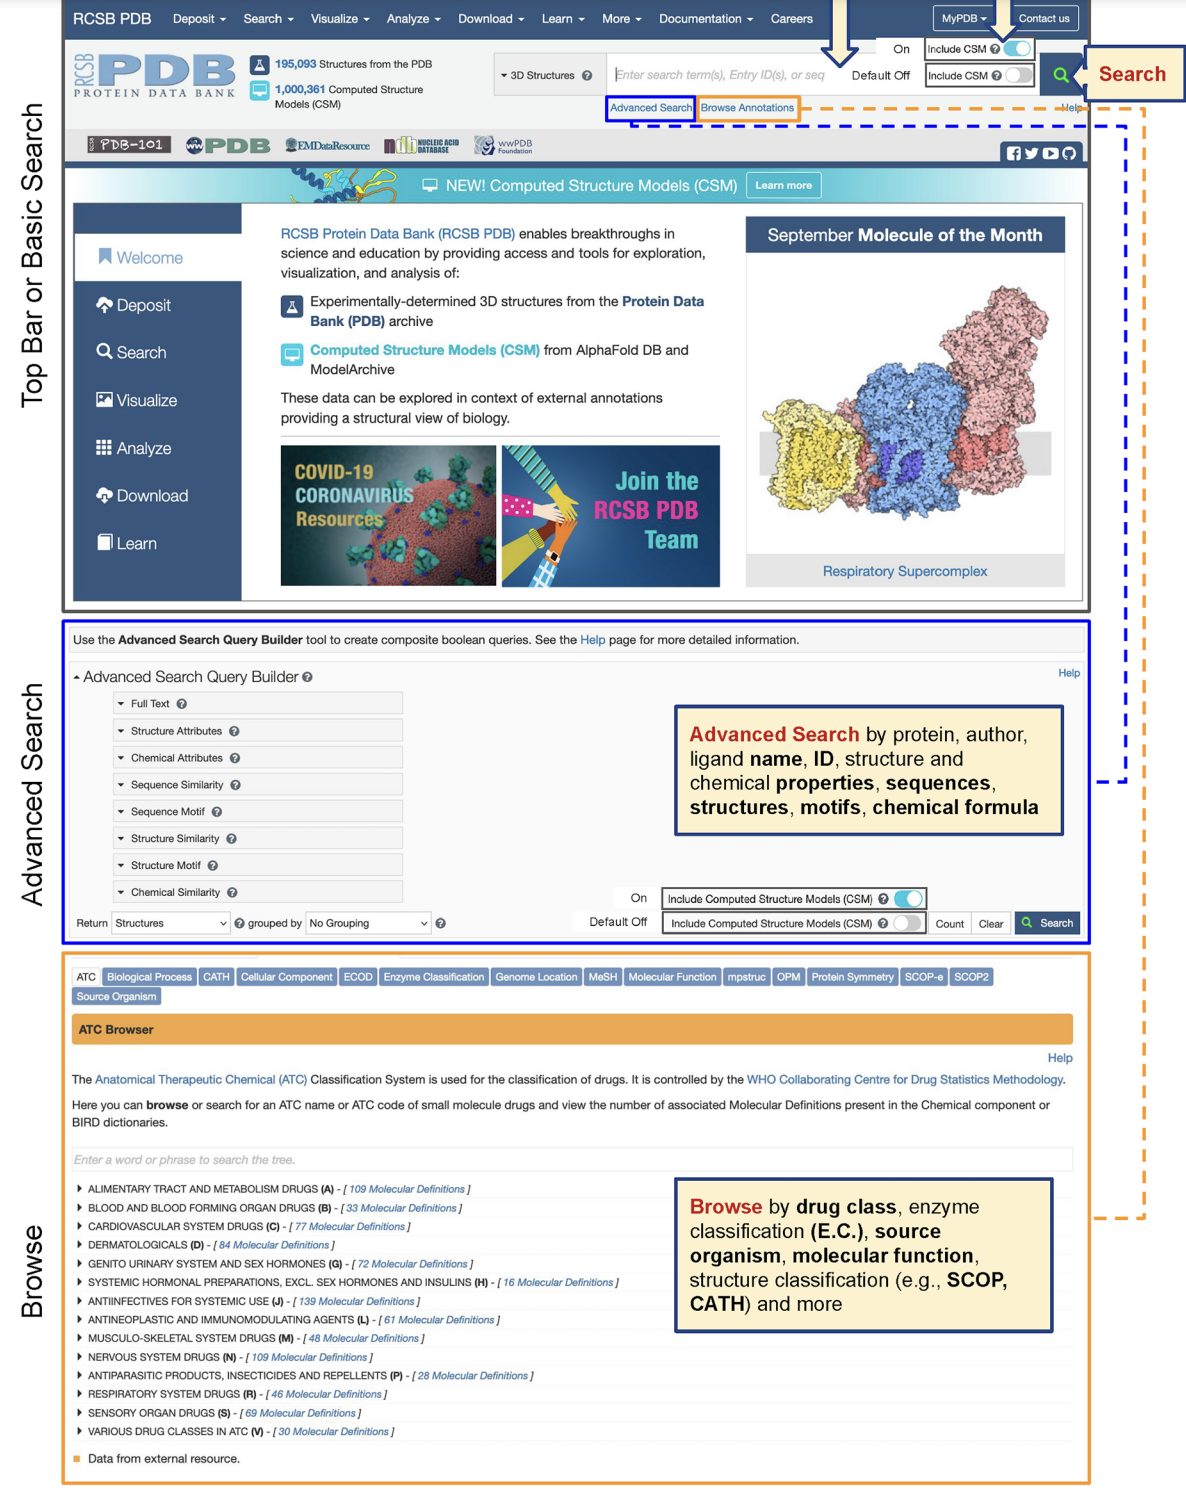
\includegraphics[width=0.5\textwidth]{PDB Site.png}
    \caption{\label{fig:PDB}Search options at RCSB.org include Top Bar or Basic Search; Advanced Search; and Browse Annotations~\cite{burley1_rcsb_2022}.}
\end{figure}

\begin{figure}[!ht]
    \centering
    \begin{subfigure}[t]{.45\textwidth}
        \centering
        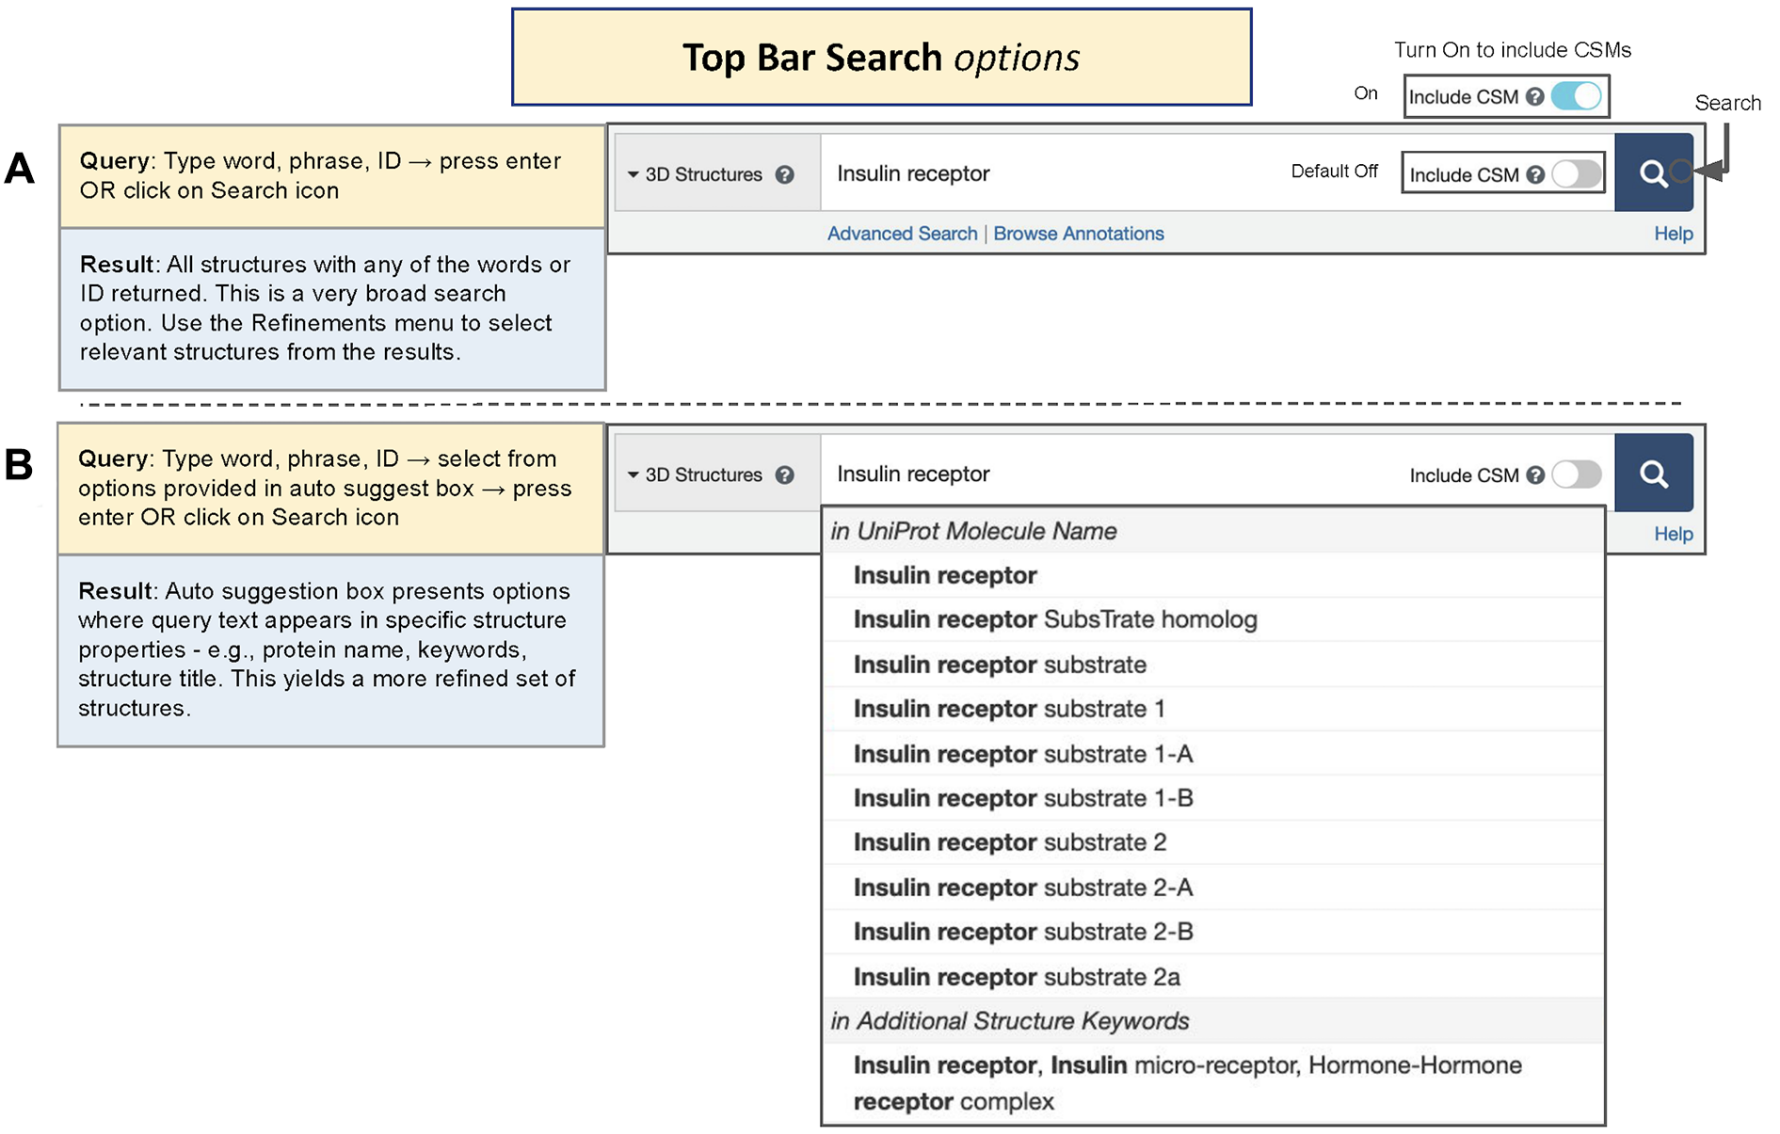
\includegraphics[width=0.9\textwidth]{Top Bar Search A.png}
        \label{fig:Top1} 
    \end{subfigure}
    \begin{subfigure}[t]{.45\textwidth}
       \centering
       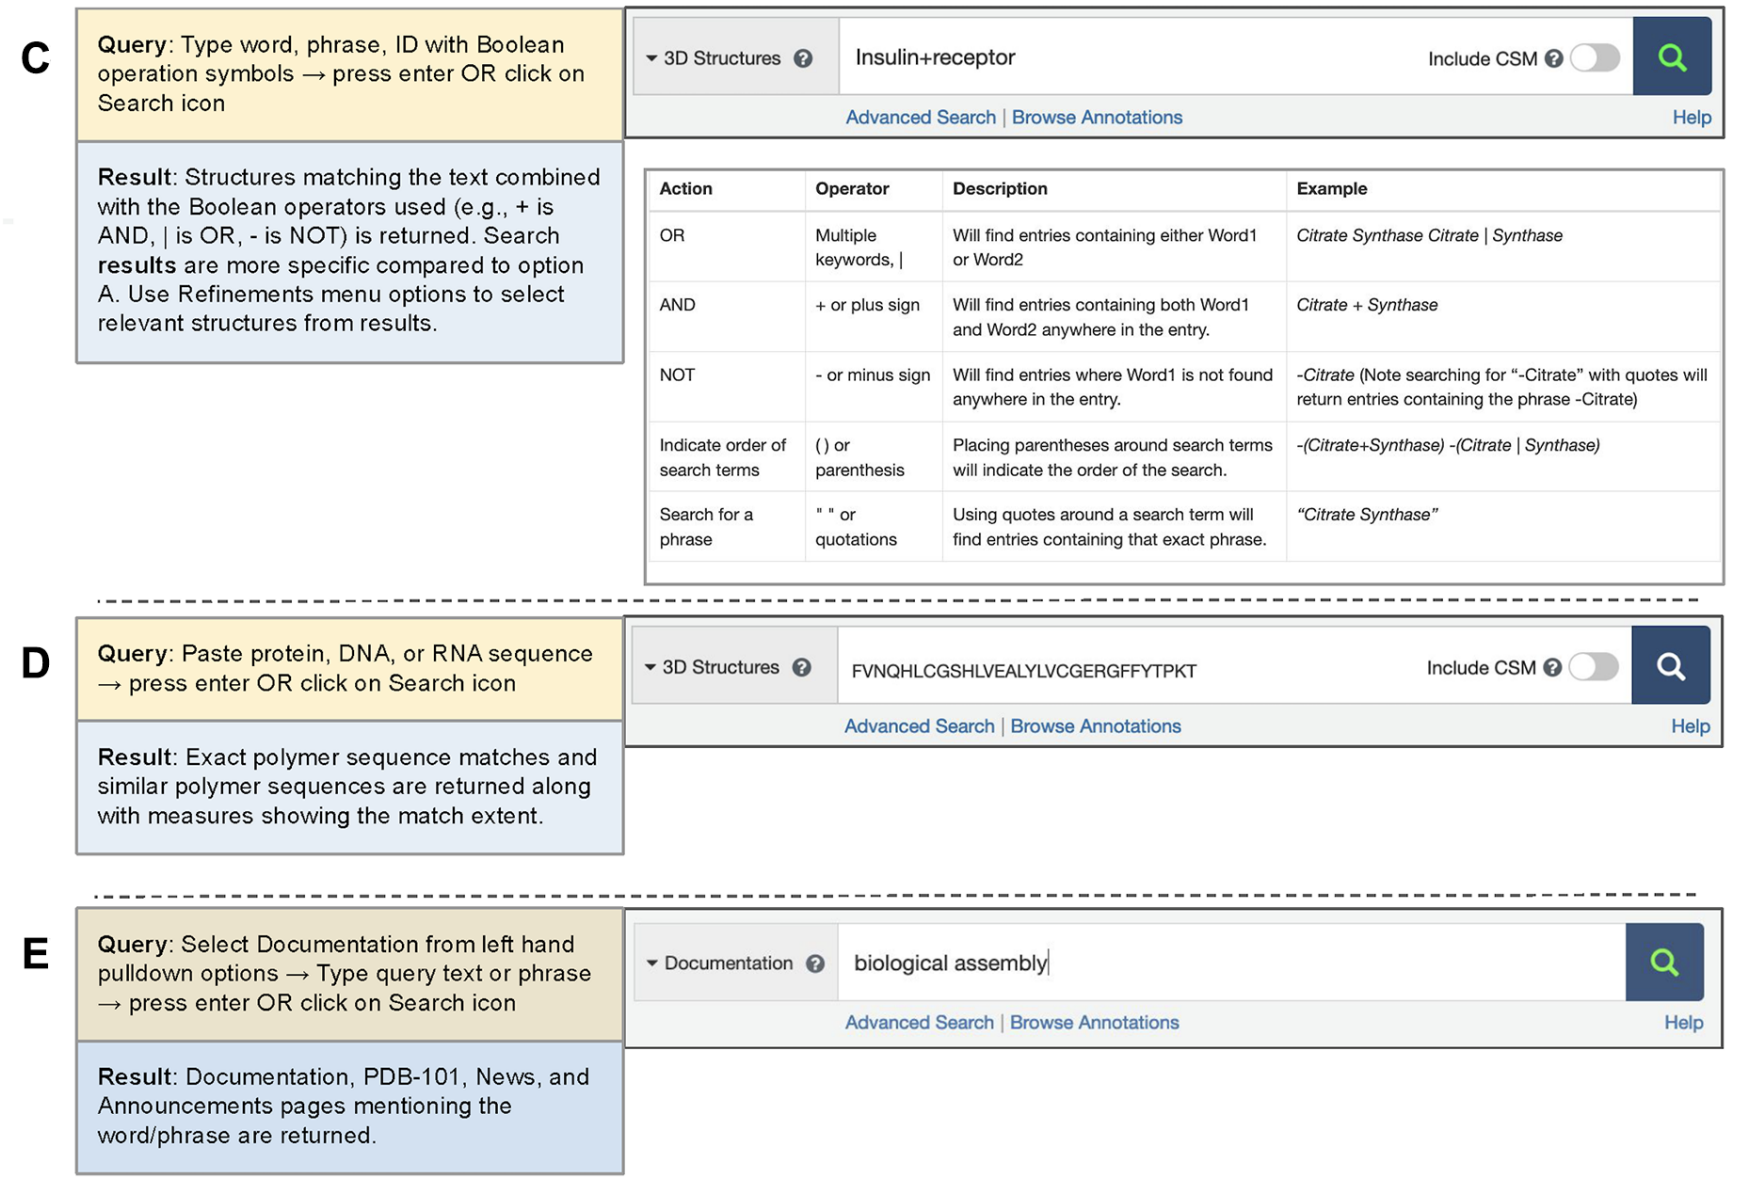
\includegraphics[width=0.9\textwidth]{Top Bar Search B.png}
       \label{fig:Top2}
    \end{subfigure}
    \caption{\emph{Top Bar or Basic Search options available from every RCSB.org web page. Examples of searching for 3D structures using (A) simple text string insulin receptor; (B) drop down autosuggestions based on the text string insulin receptor; (C) Boolean operators to combine insulin + receptor (+ = AND); or (D) an amino acid sequence. (E) Searching RCSB.org documentation using a text string biological assembly~\cite{burley1_rcsb_2022}}}
\end{figure}
\clearpage

\subsubsection{Recent RCSB PDB data architecture improvements}

In 2020, RCSB PDB had an upgrade of its delivery architecture~\cite{rose_rcsb_2021}at RCSB.org~\cite{powerful_rcsb_2021}. 

The legacy monolithic data delivery application was changed into a distributed deployment of individual microservices, each with a single responsibility. 

Data access services provide both Representational State Transfer and GraphQL API access to a data warehouse hosted in a MongoDB documentoriented database. Originally, advanced Search QueryBuilder functionality encompassed text, PDB data attributes, 3D structure, sequence, biopolymer sequence motif, and chemical similarity. Every search function is implemented as an independent service.

A separate search service is responsible for launching each search function, combining and delivering their integrated results to public programmatic search APIs. When each service has a single responsibility, we have greater flexibility in scaling the deployment of services in response to changes in user load and significant reductions in the time required to develop, test, and deploy new features. The Sequence Motif search function has been extended with a new 3D Structure Motifsearch capability~\cite{bittrich_real-time_2020}. 

\subsubsection{Recent advances in RCSB PDB data integration}

RCSB PDB integrates the content of each expertly biocurated Entry with information from more than 50 external data resources. 

Integrated external data needs to follow a data schema that defines the organization of the RCSB PDB data warehouse. Finally, it is available to RCSB PDB front-end services, public data access APIs, and our text search indexing service~\cite{burley_rcsb_2022}.

\begin{table}[h!]
    \begin{center}
    \label{tab:External Data}
        \begin{tabular}{c|p{0.58\linewidth}}
        External Resources\\
        \hline
        \\
        AlphaFold DB & Computed Structure Models by AlphaFold2
        \\
        \hline
        \\
        ATC & 	Anatomical Therapeutic Chemical (ATC) Classification System from World Health Organization
        \\
        \hline
        \\
        Binding MOAD & Binding affinities
        \\
        \hline
        \\
        Binding DB & Binding affinities
        \\
        \hline
        \\
        BMRB & BMRB-to-PDB mappings
        \\
        \hline
        \\
        Cambridge structural Database & Crystallographic small molecule data from the Cambridge Crystallographic Data Centre
        \\
        \hline
        \\
        CATH & 	Protein structure classification- Class, Architecture, Topology/fold, and Homologous superfamily    
        \\
        \hline
        \\
        ChEMBL & Manually curated database of bioactive molecules with drug-like properties
        \\
        \hline
        \\
        CSD & Cambridge Structural Database: Validated and curated small-molecule organic and metal-organic crystal structures from the Cambridge Crystallographic Data Centre
        \\
        \hline
        \\
        DrugBank & Drug and drug target data
        \\
        \hline
        \\
        ECOD & Evolutionary Classification of Protein Domains
        \\
        \hline
        \\
        EMDB & 3DEM density maps and associated metadata
        \\
        \hline
        \\
        ExplorEnz & IUBMB Enzyme nomenclature and classification
        \\
        \hline
        \\
        Gencode & Human and Mouse Gene annotations
        \end{tabular}
        \caption{\label{External Data}Some of the External Resources Integrated Into RCSB PDB}
    \end{center}
\end{table}


\subsubsection{Recent PDBx/mmCIF data standard improvements}

The PDBx/mmCIF data standard is maintained by the wwPDB organization in collaboration with wwPDBPDBx/mmCIF Working Group domain experts recruited from the scientific community. The PDBx/mmCIF web resource supports browse and search access to standard terminology. The Working Group includes developers for many of the widely used structure determination software systems, who ensure that data produced by these programs comply with the PDBx/mmCIF data standard, generating complete and correct data files for PDB deposition. The wwPDB and the Working Group collaborate on developing terminologies for new and rapidly evolving methodologies such as Free Electron Laser, 3DEM, Serial Crystallography, and X-ray, whilst improving representations for existing data content. Most recently, the Working Group has focused on modernizing content descriptions for processed X-ray diffraction data, including extensions describing anisotropic diffraction limits, unmerged reflection data, and new quality metrics of anomalous diffraction data. Deposition and delivery improve our ability to assess experimental data quality, and every PDB data consumer's ability to Find and Reuse relevant PDB Entries~\cite{burley_rcsb_2022}.

\subsubsection{Future and struggles of PDB}
\subsubsection{Future}
As the PDB archive has started its 52nd year, it gives open access to analyses of structures and much more to: basic and applied researchers, educators, and students spanning fundamental biology, biomedicine, bioenergy, bioengineering, and biotechnology, with key points that help many communities that use this facility. Firstly It delivers Data In and Data Out services efficiently to a user base that is now numbering many millions worldwide. Secondly, it has wwPDB partners that process, validate, and biocurate the growing number of increasingly complex PDB depositions received. Manages and safeguards the growing PDB archive in its role as wwPDB designated Archive Keeper. Thirdly it enables searching, visualization, exploration, and analysis of experimentally-determined PDB structures integrated with more than one million CSMs through its web portal.~\cite{burley1_rcsb_2022}.

\subsubsection{Struggles}
Even after all the advancments PDB has gone through there are still additional challenges lying ahead which include:

\begin{itemize}
    \item Rapid growth in public-domain CSMs of individual polypeptide chains, already numbering >200 million at the time of writing.
    \item Anticipated advances in AI/ML-based prediction of structures of multi-protein complexes.
    \item Continued development of biomolecular structure determination methods using X-ray Free Electron Lasers, revealing the microscopic details of chemical reactions in real time.
    \item Growth in the number and complexity of atomic-level cryoelectrontomography structures of macromolecular machines.
    \item Integration of PDB structures and CSMs with complementary information coming from correlative light microscopy and related imaging methods across length scales ranging from atoms to small molecules to individual biomolecules to macromolecular assemblies to organelles to cells and ultimately tissues
    \item Merging of the PDB-Dev prototype archiving system for integrative methods structures with the PDB archive
    \item Federating other biodata resources, such as the SmallAngle Scattering Database and the Proteomics Identification Database, with the PDB, EMDB and BMRB core archives jointly managed by the wwPDB partnership
\end{itemize}
~\cite{burley1_rcsb_2022}.

\subsubsection{File Formats}

The PDB archive holds a few different types of file types that hold data such as atomic coordinates and other information describing proteins and other biological macromolecules. Depending on what the data is created from it can fall into a different category.

\subsubsection{PDB Data}

The main information in the PDB archive is coordinate files for biological molecules. These files list the atoms in each protein and their 3D coordinates.

These files are available in several formats:

\begin{itemize}
    \item PDB
    \item mmCIF
    \item XML
\end{itemize}

The header section of the text summarizes the protein, citation information, and the details of the structure solution, which is then followed by the sequence and a long list of the atoms and their coordinates. It also contains the experimental observations used to determine atomic coordinates~\cite{noauthor_pdb101_nodate}.

\subsubsection{.pdb Files}

The PB format consists of a collection of records that describe the atomic coordinates, chemical and biochemical features, and experimental details of the structure determination~\cite{westbrook_pdb_2003}.

Each item of data in the PDB format is assigned to a one of PDB record types (HEADER. SOURCE. REMARK, etc.). The ATOM records the atomic coordinate data~\cite{westbrook_pdb_2003}.

PDB format has been extended with new REMARK records. For example, REMARK 3 that encodes refinement information has been modified and extended for each new refinement program and program version~\cite{westbrook_pdb_2003}.

The PB format uses fixed-width fields to represent data, so we have limits on the size of certain items of data. For example, we cant have more then 99,999 atoms and polymer chain can be only one character. This means some structures are devided into multiple files~\cite{westbrook_pdb_2003}.

\begin{figure}[ht]
    \centering
    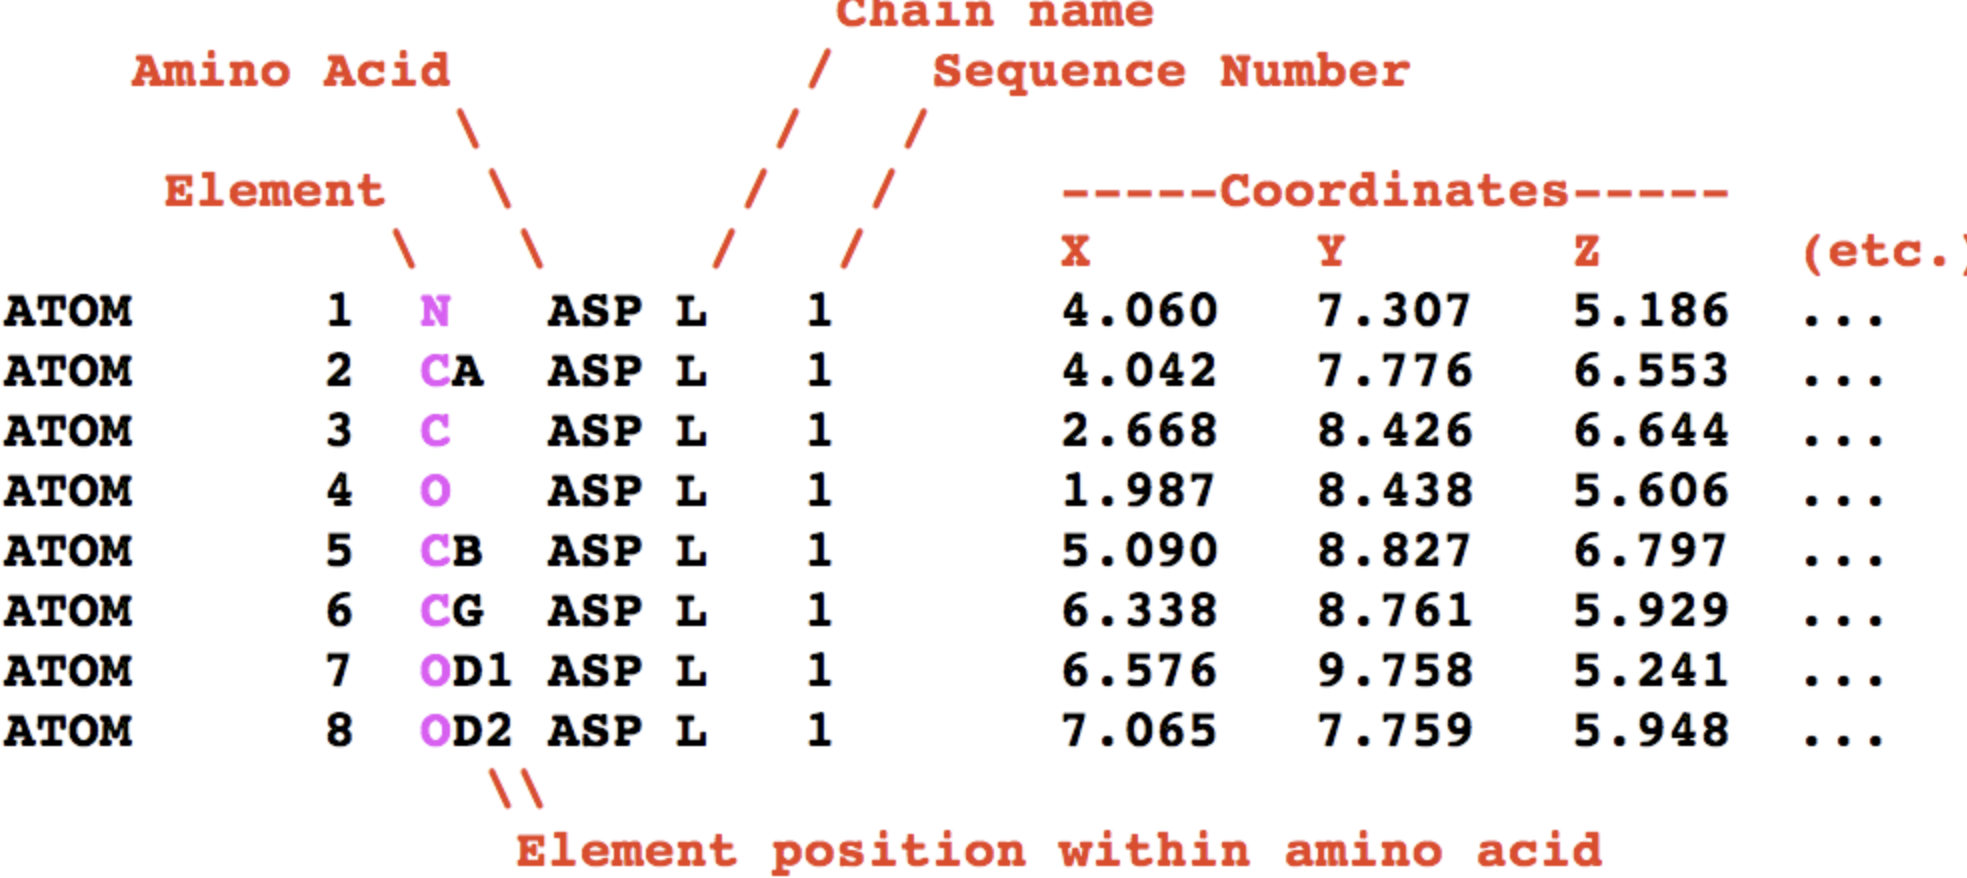
\includegraphics[width=0.5\textwidth]{PDB File.png}
    \caption{\label{fig:PDB file}Showing contents of a PDB file for the Atom values~\cite{adams_announcing_2019}.}
\end{figure}

\subsubsection{.mmCIF Files}
Mmcif is a dictionary-based approach to data extracted from crystallographic experiments~\cite{westbrook_pdb_2003}.

It includes all the data we can find in a pdb file. Also, we have sufficient data names so that the experimental section of a structure paper can be written automatically and to facilitate the development of tools i.e. computer programs could easily access and validate mmCIF data files~\cite{westbrook_pdb_2003}.

\subsubsection{.xml}

XML builds from a PDB Exchange dictionary. Although presented in very different syntaxes, the PDB Exchange and XML representations use the same logical data organization.~\cite{westbrook_pdbml_2005}.

The dictionary data block is mapped to the standard top-level XML schema element, and the data file data block is mapped to a datablock element. Category or table definitions in the Exchange dictionary are described as XML complex types. The category definition.~\cite{westbrook_pdbml_2005}.

\begin{figure}[ht]
    \centering
    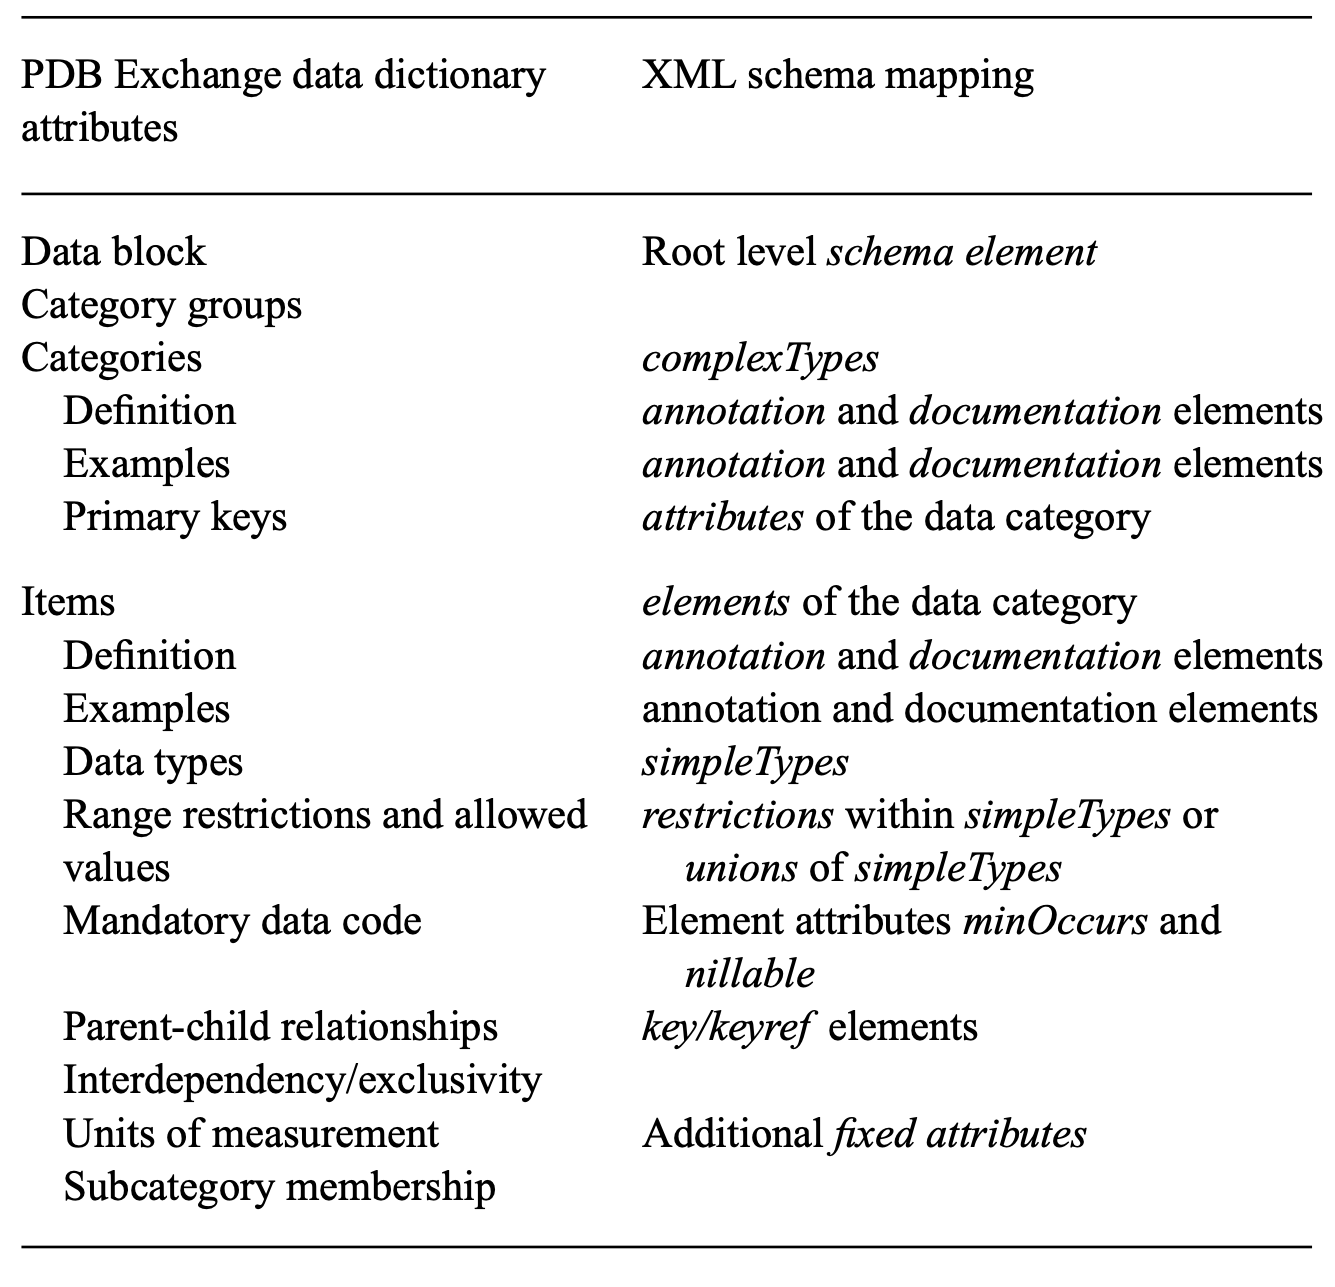
\includegraphics[width=0.5\textwidth]{xml.png}
    \caption{\label{fig:xml}Summary of the correspondences between PDB Exchange data dictionary and XML schema metadata~\cite{westbrook_pdbml_2005}.}
\end{figure}


\subsubsection{Visualizing Structures}

PDB files can be viewed from text editors but we can also use a browsing or visualization program. RCSB PDB allows you to search and explore the information, including information on experimental methods and the chemistry and biology of the protein. Visualization programs allow to read of the PDB file and, display the protein structure generating custom pictures of it. These programs can contain analysis tools that allow you to measure distances and bond angles, and identify interesting structural features~\cite{noauthor_pdb101_nodate}.

\subsubsection{Reading Coordinate Files}

Before exploring structures in the PDB archive we need some prior understanding of the coordinate files. For example, we can find a diverse mixture of biological molecules, small molecules, ions, and water which can get confusing we can use the names and chain IDs to help sort these out. In structures determined from crystallography, atoms are annotated with temperature factors that describe their vibration and occupancies that show if they are seen in several conformations. NMR structures often include several different models of the molecule~\cite{noauthor_pdb101_nodate}.

\subsubsection{Potential Challanges}

There are some things to note as you could fall into some challenges when browsing through the PDB archive. Many structures, particularly those determined by crystallography, only include information about part of the functional biological assembly. One thing to note is that the PDB can aid with this. Another note is many PDB entries are missing portions of the molecule that were not observed in the experiment. These include structures that include only alpha carbon positions, structures with missing loops, structures of individual domains, or subunits from a larger molecule. In addition, most of the crystallographic structure entries do not have information on hydrogen atoms~\cite{noauthor_pdb101_nodate}.

\subsection{Hadoop spark and pyspark}

\subsubsection{What is Hadoop}

Hadoop is an open-source framework for writing and running distributed applications that process large amounts of data.  Key aspects making it valuable such 1. Accessible 2.Robust 3. Scalable 4.simple~\cite{lam_hadoop_2010}.

HDFS is used in haddop which is a filessystem and a MapReduce engine. With one master node and many worker nodes. The master node provides instructions to the worker nodes and computations are performed on the worker nodes.~\cite{hazarika_performance_2017}.

\subsubsection{Mapper}
Input key/value pairs are mapped to a set of key/value pairs. The mapper then sorts the key-value pairs by the keys. Partitioners are mainly responsible for providing intermediate key/values to the reducers~\cite{patel_addressing_2012}~\cite{hazarika_performance_2017}.

\subsubsection{Reducer}

Firstly, the reducer combines data having the same key from different map functions. The values having the same key are reduced to a smaller set of values and output is produced~\cite{hazarika_performance_2017}.

\subsubsection{What is Spark}
Apache Spark is a popular open-source platform for large-scale data processing used for iterative machine learning tasks~\cite{meng_mllib_2016}.

Spark is a cluster computing system providing APIs in Java, Scala, Python (pySpark), and R, along with an optimized engine that supports general execution graphs. Moreover, Spark is efficient at iterative computations so it is suited for the development of large-scale machine learning applications~\cite{meng_mllib_2016}.

Spark is a quick and general engine used for analysing large-scale data stored across a cluster of computers. Spark uses in-memory cluster computing which is its most important feature for increasing the processing speed of an application. It combines SQL streaming and complex analytics~\cite{hazarika_performance_2017}.

\subsubsection{Spark Architecture}

There are five core components that make Spark so powerful and easy to use. The core architecture of Spark consists of the following layers:

\begin{itemize}
    \item Storage
    \item Resource management
    \item Engine
    \item Ecosystem
    \item APIs
\end{itemize}
~\cite{singh_manage_2022}.
\subsubsection{Storage}
Before using Spark, data must be made available in order to process it. This data can reside in any kind of database. Spark offers multiple options to use different categories of data sources, to be able to process it on a large scale. Spark allows you to use traditional relational databases as well as NoSQL, such as Cassandra and MongoDB~\cite{singh_manage_2022}.

\subsubsection{Resource Management}
The next layer consists of a resource manager. As Spark works on a set of machines (it also can work on a single machine with multiple cores), it is known as a Spark cluster. Typically, there is a resource manager in any cluster that efficiently handles the workload between these resources. The two most widely used resource managers are YARN and Mesos. The resource manager has two main components internally~\cite{singh_manage_2022}:

\begin{itemize}
    \item Cluster manager
    \item Worker
\end{itemize}

It’s kind of like master-slave architecture, in which the cluster manager acts as a master node, and the worker acts as a slave node in the cluster. The cluster manager keeps track of all information pertaining to the worker nodes and their current status. Cluster managers always maintain the following information~\cite{singh_manage_2022}:

\begin{itemize}
    \item Status of worker node (busy/available)
    \item Location of worker node
    \item Memory of worker node
    \item Total CPU cores of worker node
\end{itemize}

The main role of the cluster manager is to manage the worker nodes and assign them tasks, based on the availability and capacity of the worker node. On the other hand, a worker node is only responsible for executing the task it’s given by the cluster manager~\cite{singh_manage_2022}.

The tasks that are given to the worker nodes are generally the individual pieces of the overall Spark application. The Spark application contains two parts~\cite{singh_manage_2022}:

\begin{itemize}
    \item Task
    \item Spark driver
\end{itemize}

The task is the data processing logic that has been written in either PySpark or Spark R code. It can be as simple as taking a total frequency count of words to a very complex set of instructions on an unstructured dataset. The second component is Spark driver, the main controller of a Spark application, which consistently interacts with a cluster manager to find out which worker nodes can be used to execute the request. The role of the Spark driver is to request the cluster manager to initiate the Spark executor for every worker node~\cite{singh_manage_2022}.

\subsubsection{Engine and Ecosystem}

The base of the Spark architecture is its core, which is built on top of RDDs (Resilient Distributed Datasets) and offers multiple APIs for building other libraries and ecosystems by Spark contributors. It contains two parts: the distributed computing infrastructure and the RDD programming abstraction. The default libraries in the Spark toolkit come as four different offerings~\cite{singh_manage_2022}.

\subsubsection{Spark SQL}

SQL being used by most of the ETL operators across the globe makes it a logical choice to be part of Spark offerings. It allows Spark users to perform structured data processing by running SQL queries. In actuality, Spark SQL leverages the catalyst optimizer to perform the optimizations during the execution of SQL queries. Another advantage of using Spark SQL is that it can easily deal with multiple database files and storage systems such as SQL, NoSQL, Parquet, etc~\cite{singh_manage_2022}.

\subsubsection{MLlib}

Training machine learning models on big datasets was starting to become a huge challenge, until Spark’s MLlib (Machine Learning library) came into existence. MLlib gives you the ability to train machine learning models on
huge datasets, using Spark clusters. It allows you to build in supervised, unsupervised, and recommender systems; NLP-based models; and deep learning, as well as within the Spark ML library~\cite{singh_manage_2022}.

\subsubsection{Structured Streaming}

The Spark Streaming library provides the functionality to read and process real-time streaming data. The incoming data can be batch data or near real-time data from different sources. Structured Streaming is capable of ingesting real-time data from such sources as Flume, Kafka, Twitter, etc~\cite{singh_manage_2022}.

\subsubsection{Graph X}

This is a library that sits on top of the Spark core and allows users to process specific types of data (graph dataframes), which consists of nodes and edges. A typical graph is used to model the relationship between the different objects involved. The nodes represent the object, and the edge between the nodes represents the relationship between them. Graph dataframes are mainly used in network analysis, and Graph X makes it possible to have distributed processing of such graph dataframes~\cite{singh_manage_2022}.

\subsubsection{Programming Language APIs}

Spark is available in four languages. Because Spark is built using Scala, that becomes the native language. Apart from Scala, we can also use Python, Java, and R~\cite{singh_manage_2022}.

\subsubsection{Spark Execution}

Any Spark application spins off a single driver process (that can contain multiple jobs) on the master node that then directs executor processes (that contain multiple tasks) distributed to a number of worker nodes shown ~\ref{fig:Execute.png}.

\begin{figure}[ht]
    \centering
    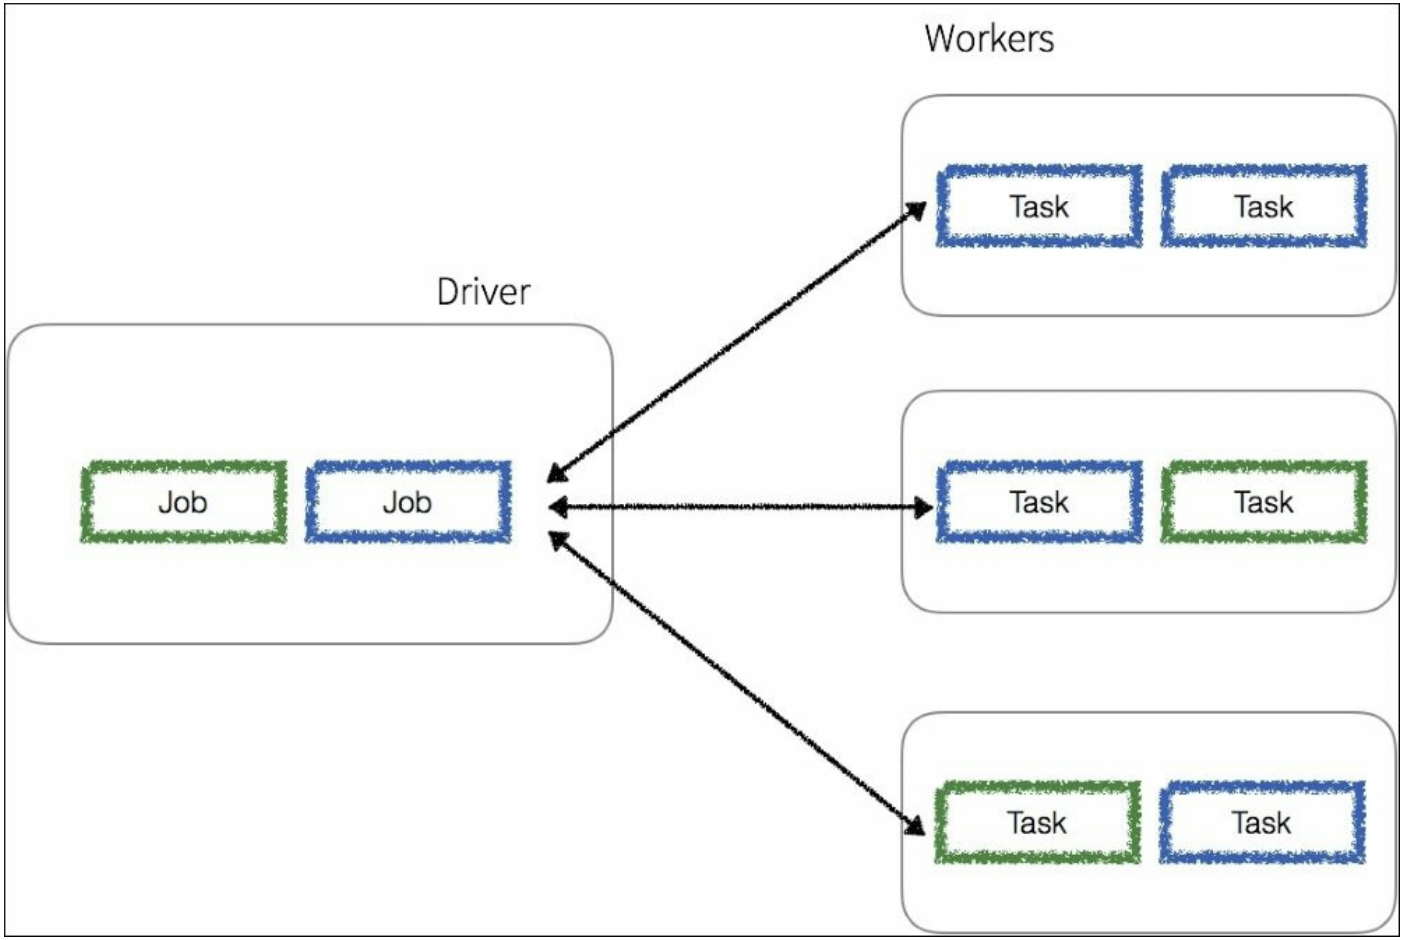
\includegraphics[width=0.5\textwidth]{Execute.png}
    \caption{\label{fig:Execute.png}Think of somthing to say~\cite{drabas_learning_2017}.}
\end{figure}


The driver process determines the number and the composition of the task processes directed to the executor nodes based on the graph generated for the given job. Note, that any worker node can execute tasks from a number of different jobs~\cite{drabas_learning_2017}.

\subsubsection{Spark vs Hadoop}

\begin{table}[ht!]
    \begin{center}
    \label{tab:Amino acids}
        \begin{tabular}{p{0.6\linewidth}|p{0.35\linewidth}}
        Hadoop Map Reduce & Spark\\
        \hline
        \\
        For Applications that repeatedly reuse the same set of data, map reduce is very inefficient. & Spark uses in-memory processing, reusing it for faster computation.
        \\
        \hline
        \\
        MapReduce is quite faster in batch processing. & As memory size is limited, it would be quite slower in batch processing of huge data set.
        \\
        \hline
        \\
        Data is stored in disk for processing. & Data is stored in main memory. As it is an inmemory computation engine entire data is copied. 
        \\
        \hline
        \\
        Difficulty in processing and modifying data in real time due to its high latency. & Used to process and modify data in real time due to its low latency. 
        \\
        \hline
        \\
        Predominantly used to process from bygone datasets. & Predominantly used for streaming, batch processing and machine learning
        \\
        \hline
        \\
        For fault tolerance, MapReduce uses replication. & For fault tolerance, Spark uses RDDs.
        \\
        \hline
        \\
        It merges and partitions shuffle files. & It does not merges and partition shuffle files. 
        \\
        \hline
        \\
        Primarily disk based computation. & Primarily RAM based computation.
        \\
        \end{tabular}
        \caption{\label{hadoopvsspark}Showing the differences between haddop and spark~\cite{hazarika_performance_2017}.}
    \end{center}
\end{table}

\begin{table}[ht!]
    \begin{center}
    \label{tab:Amino acids}
        \begin{tabular}{c|cc}
        Number of words & Hadoop (Sec) & Spark(Sec)\\
        \hline
        \\
        100 & 79 & 28.841
        \\
        1000 & 91 & 31.185
        \\
        10000 & 96 & 35.181
        \\
        100000 & 103 & 36.969
        \\
        1000000 & 116 & 39.569
        \end{tabular}
        \caption{\label{Results1}Comparision of Execution time for wordcount program~\cite{hazarika_performance_2017}.}
    \end{center}
\end{table}

\begin{table}[ht!]
    \begin{center}
    \label{tab:Amino acids}
        \begin{tabular}{c|cc}
        Number of words & Hadoop (Sec) & Spark(Sec)\\
        \hline
        \\
        5 & 2.541 & 0.9030
        \\
        10 & 3.370 & 1.459
        \\
        50 & 6.420 & 2.840
        \\
        100 & 9.383 & 3.452
        \\
        200 & 10.100 & 5.749 
        \end{tabular}
        \caption{\label{Results1}Comparison of Execution time for logistic
        regression program~\cite{hazarika_performance_2017}.}
    \end{center}
\end{table}

Summarising the results shows Spark to be quicker in both experiments. Spark also provides an API for python which will be very helpful in this project seeing its easy nature to be able to read files and work with text-based files. Therefore I have decided to work with Pyspark for this project.

\subsubsection{Software Architectural Bottlenecks}

HDFS has scheduling delays in the architecture which results in cluster nodes waiting for new tasks as the access pattern is periodic.HDFS client code, serializes computation and I/O instead of decoupling and pipelining those operations.~\cite{shafer_hadoop_2010}.

\begin{definition}[HDFS]
    The Hadoop Distributed File System (HDFS) is a distributed file system designed to run on commodity hardware
\end{definition}

\subsubsection{Portability Limitations}
Some performance-enhancing features in the filesystem are not available such as bypassing the filesystem page cache and transferring data directly from the disk into user buffers. Thus, HDFS implementation runs less efficiently and has higher processor usage than would otherwise be necessary~\cite{shafer_hadoop_2010}.

\subsection{Analysis of existing systems that solve similar tasks}
There are a few systems that solve similar tasts these include:

\begin{itemize}
    \item SparkMD: This is a Spark-based framework for molecular dynamics simulations. It uses a distributed version of the GROMACS simulation engine to enable large-scale simulations of protein systems.
    \item BioSpark: This is a Spark-based framework for processing and analyzing large-scale genomics and proteomics datasets. It provides a set of APIs for analyzing DNA sequences, protein structures, and other biological data.
    \item Pysparkling: This is a Python-based library for parallelizing computations using Spark. It can be used for a range of bioinformatics analyses, including sequence alignment, protein structure prediction, and gene expression analysis.
    \item SparkProt: This is a Spark-based framework for protein structure prediction. It uses a combination of machine learning algorithms and structural bioinformatics tools to predict the 3D structure of proteins from their amino acid sequences.
    \item DeepChem: This is a deep learning-based framework for drug discovery and development. It uses Spark to parallelize computations and can be used for a range of tasks, including protein-ligand docking, virtual screening, and compound synthesis planning.
\end{itemize}


\section{Everything Below i would like to expand on more will be doing so as my next steps}


\section{Software Engineering}
\subsection{Objective Implementation}

\begin{itemize}
    \item Develop a software framework that suppots the Mapreduce formalism and can process
    large numbers of protein structures.
\end{itemize}

To implement this we need to break down the objective into two parts the first part is to achieve a framework that supports a mapreduce formalism. In order to do this i need to decide between hadoop and apache spark. Please refer to my Literature review on Hadoop spark and pyspark where spark performes quicker whilst having having an API for python.

\subsubsection{Implementing PySpark}

Install Java: PySpark requires Java to run. You can download and install the latest version of Java from the official website (https://www.oracle.com/java/technologies/javase-downloads.html).

Install Apache Spark: PySpark is built on top of Apache Spark, so you need to install Apache Spark first. You can download the latest version of Apache Spark from the official website (https://spark.apache.org/downloads.html). Choose a pre-built package for Apache Spark and select the version that matches your installed Java version. Extract the downloaded package to a location of your choice.

Install Python: PySpark requires Python 3.x to run. You can download and install the latest version of Python from the official website (https://www.python.org/downloads/).

Set environment variables: To use PySpark, you need to set environment variables for Java and Spark. As I am implementing this on MAC OS to do so we need to open the terminal and run the following commands:

\begin{lstlisting}[language=bash]
    export JAVA_HOME=/Library/Java/JavaVirtualMachines/<JDK_version>/Contents/Home
    export PATH=$JAVA_HOME/bin:$PATH
    export SPARK_HOME=<path_to_spark_folder>
    export PATH=$SPARK_HOME/bin:$PATH
\end{lstlisting}

Replace 'JDK version' with the version of Java you installed and 'path to spark folder' with the path to the folder where you extracted Apache Spark.

Install PySpark: You can install PySpark using pip. Open the terminal and run the following command:

\begin{lstlisting}[language=bash]
    pip install pyspark
\end{lstlisting}

Finally Test PySpark: You can test PySpark to check if all is set uop correctly by opening the Python shell and running the following commands:

\begin{lstlisting}[language=bash]
    from pyspark.sql import SparkSession
    spark = SparkSession.builder.appName("test").getOrCreate()
    df = spark.range(10)
    df.show()
\end{lstlisting}

This should create a Spark session, create a DataFrame with 10 rows, and display it in the console.

The second part of the objective is to ensure that we can process large numbers of protein structures. To do this we need to optimize our Spark job and cluster configuration. There are some actions we can not implement, some actions we can consider before the code and finally  some actions we can implement in to our code.

\subsubsection{Can not implement}
We can not implemnet this in to our project as it has been decided that the framework will stick to one node in a local cluster and use better serlizatition formats due to the time constraints.

Cluster Configuration:
Make sure that you have a cluster with sufficient resources to handle the amount of data you want to process. You can use Amazon EMR, Google Cloud Dataproc or any other cloud-based solution to spin up a cluster with adequate resources.

Data Serialization:
Serialization is the process of converting data structures into a format that can be easily transmitted over the network. By default, PySpark uses Python's pickle library for serialization, which can be slow for large datasets. You can improve serialization performance by using more efficient serialization formats like Avro or Parquet.

\subsubsection{Before implementing the code}
Hardware Configuration:
Ensure that your cluster has sufficient CPU, RAM, and disk resources to handle the workload. You can also use SSDs (Solid State Drives) for faster disk access and faster I/O operations.

To do this we need to look at the minimum requirements for running PySpark.

\begin{itemize}
    \item A 64-bit operating system e.g., macOS, Linux, or Windows
    \item At least 8 GB of RAM
    \item A multi-core processor e.g., Intel Core i5 or i7
\end{itemize}

\subsubsection{Whilst Implementing code}
These are some functions that we can implement into our code to ensure that optimize our Spark job and cluster configuration
Partitioning:
Partitioning the input data can significantly improve performance, especially for large datasets. Partitioning involves splitting the data into smaller chunks and processing them in parallel. You can specify the number of partitions using the repartition function in PySpark.

Caching:
Caching is an optimization technique that involves storing intermediate results in memory to avoid recomputation. Caching is particularly useful when you have iterative algorithms that reuse the same data multiple times. You can use the cache function in PySpark to cache Resilient Distributed Datasets or DataFrames.\\\\

\begin{itemize}
    \item Implement a distributed computing system using MapReduce to parallelize protein
    structure analysis across multiple computing nodes.
\end{itemize}

To implement a distributed computing system using MapReduce to parallelize protein structure analysis across multiple computing nodes using PySpark, we need complete the following steps:

\begin{enumerate}
    \item Setup a PySpark cluster with multiple worker nodes.
    \item Write a Map function to parse the protein structure data and extract the relevant features.
    \item Write a Reduce function to combine the results from the Map function.
    \item Load the protein structure data into PySpark RDDs.
    \item Apply the Map function to each protein structure RDD in parallel.
    \item Apply the Reduce function to combine the results from the Map function.
    \item Save the output to a distributed file system.
\end{enumerate}

The following code has been taken from my lines program which is inteanded to print the number of lines each pdb file contains which complete the steps above

\begin{lstlisting}
    from pyspark.sql import SparkSession
    from pyspark.sql.types import StringType
    import os
    from pathlib import Path
    import tempfile

    def main(spark):
        directory = ("/Users/vinaykakkar/Desktop/PROJECT/Programs/Lines/PDBsDirectory/*")
        tempdirectory = "/Users/vinaykakkar/Desktop/PROJECT/Programs/Lines/PDBsfromRDD"

        rddkeyvalue = spark.sparkContext.wholeTextFiles(directory)

        def numberoflines(filename, filecontent):
            with tempfile.NamedTemporaryFile(prefix=filename[69:], mode='w') as tmp:
                tmp.write(filecontent)
                os.system("wc -l "+ tmp.name)

        rddkeyvalue.map(lambda x: numberoflines(x[0], x[1])).collect()

    if __name__ == '__main__':
        spark = SparkSession.builder.appName('PDB').getOrCreate()
        main(spark)

\end{lstlisting}

\subsubsection{PySpark cluster setup}

The SparkSession object is a higher-level interface to create a Spark application with SparkContext, which provides a unified entry point to interact with the Spark cluster.

We use the builder API to create a SparkSession instance and set the application name to "PDB". The getOrCreate method creates a new SparkSession instance or reuses an existing one if one already exists. This creates a SparkSession with all the necessary configurations and settings for connecting to the Spark cluster.

When we execute the code, the SparkSession instance is created and the worker nodes are launched, enabling distributed computing across the cluster.

\subsubsection{Map function}
The numberoflines function takes a folders path and the values within the protien structure and creates a temp file in which it writes the contents of the protien structure. The temp file is then used to get the number of lines with the shell command "wc -l 'tempfilename'".

Once the numberoflines function has been defined, we can apply it to each protein structure file in parallel using the Map function in Spark.


\subsubsection{Reduce function}
The code provided does not include an explicit implementation of a Reduce function. However, you can write a Reduce function using PySpark's reduce function, which would result in the same respone if needed to return the number of lines.

\subsubsection{PySpark RDDs}
The code provided loads protein structure data by using the wholeTextFiles function to read in all the files in a directory as an RDD of key-value pairs, where the key is the filename and the value is the contents of the file.

\subsubsection{Save to distributed file system}
The code provided does not include any code to save the output to a distributed file system. However, you can use PySpark's saveAsTextFile function to save the output as text files in a distributed file system.

\begin{itemize}
    \item Optimize the software framework to reduce the processing time required for protein structure analysis.
\end{itemize}

I will now present the first version of my lines programs and explain features i changed so that the framework will be more optimized for reduce the processing time required for protein structure analysis.

\begin{lstlisting}
    from pyspark.sql import SparkSession
    from pyspark.sql.types import StringType
    import os
    import shutil
    from pathlib import Path


    def main(spark):
        directory = ("/Users/vinaykakkar/Desktop/PROJECT/Programs/Lines/PDBsDirectory")
        tempdirectory = "/Users/vinaykakkar/Desktop/PROJECT/Programs/Lines/PDBsfromRDD"

        for file in os.listdir(os.fsencode(directory)):
            filename = os.fsdecode(file)
            if filename.endswith(".DS_Store"):
                continue
            rdd = spark.read.text("Programs/Lines/PDBsDirectory/"+filename).rdd.map(lambda x: x[0])
            if os.path.exists(tempdirectory):
                shutil.rmtree(tempdirectory)
            rdd.saveAsTextFile(tempdirectory)
            os.system("wc -l "+tempdirectory+"/part-00000")


    if __name__ == '__main__':
        # This creates a local cluster
        spark = SparkSession.builder.appName('PDB').getOrCreate()
        main(spark)
\end{lstlisting}

\subsubsection{Issues with code}
We have instasiated a for loop which loops through all the files in the PDBsDirectory the code then reads each file in the PDBsDirectory directory and loads it into an RDD using spark.read.text ignoring any files that end with DSStore which is one of the outputs returned from saveAsTextFile. This operation can be time-consuming for large files because it involves reading the entire file into memory as a single string. This is not efficient for processing large files.

The code then saves the RDD to the PDBsfromRDD directory using rdd.saveAsTextFile but we need to check if this directory exists already, deleting it if so, as for the next pdb file in the PDBsDirectory we will need to cast saveAsTextFile to this which requires that folder to not exist in the first place. SaveAsTextFile function can be expensive because it involves writing the entire RDD to disk.

Finally if there is a lot of files in PDBsDirectory the the for loop will need to go through each one whilst also running shutil.rmtree which is not effeciant as there are some operations being run each iteration which we can remove.

\subsubsection{Improvment Using wholeTextFiles()}

wholeTextFiles() can be used instead of textFile() to read all files within a directory as a single RDD. wholeTextFiles() reads the files in the specified directory and returns an RDD where each element is a tuple of (filename, contents), where filename is the name of the file and contents is the entire contents of the file as a single string.

This eliminates the need to have a for loop to go through the directory as we can read each file in the directory using wholeTextFiles() and a wildcard '*' in the directory path for example directory = "/path/*" which will select all the files in that path.

As we have the name and content of the file we can remove saveAsTextFile() as we can pass in the file name into the map function thus casting the shell command on the file.

This will result in the following code:

\begin{lstlisting}
    from pyspark.sql import SparkSession
    from pyspark.sql.types import StringType
    import os
    import shutil
    from pathlib import Path


    def main(spark):
        start = time.time()
        directory = ("/Users/vinaykakkar/Desktop/PROJECT/Programs/Lines/PDBsDirectory/*")

        rddkeyvalue = spark.sparkContext.wholeTextFiles(directory)

        def numberoflinesinfile(k):
            os.system("wc -l "+ k[40:])
        
        rddkeyvalue.map(lambda x: numberoflinesinfile(x[0])).collect()


    if __name__ == '__main__':
        # This creates a local cluster
        spark = SparkSession.builder.appName('PDB').getOrCreate()
        main(spark)

\end{lstlisting}

\begin{itemize}
    \item Validate the software framework by testing it with a variety of protein structure analysis tools and evaluating its performance in comparison to other available tools.
\end{itemize}

\subsubsection{Need help with the above bullet point not sure what to write about}

\begin{itemize}
    \item Design an interface that allows users to manipulate the pdbs that are being passed into
    the executable for protein structure analysis.
\end{itemize}

\subsubsection{Need to hold out on this one as we could potentially have a ui}

\begin{itemize}
    \item Ensure the software framework is scalable and can handle increasingly large datasets.
\end{itemize}

There are several things we can consider to esnure the software framework is scalable and can handle increasingly large datasets:

\begin{enumerate}
    \item Partitioning data
    \item Distributed computing
    \item Efficient algorithms
    \item Testing and validation
\end{enumerate}

I will be using my TMalign program to show how i have implemented each one of these:


\begin{lstlisting}
    def main(spark):
        directory1 = ("/Users/vinaykakkar/Desktop/PROJECT/Programs/TMalign/PDBsDirectory1/*")
        directory2 = ("/Users/vinaykakkar/Desktop/PROJECT/Programs/TMalign/PDBsDirectory2/*")

        rddkeyvalue1 = spark.sparkContext.wholeTextFiles(directory1)
        rddkeyvalue2 = spark.sparkContext.wholeTextFiles(directory2)

        rdd = rddkeyvalue1.cartesian(rddkeyvalue2)

        def runTMalign(tuple1, tuple2):
            with tempfile.NamedTemporaryFile(prefix = tuple1[0][72:], mode='w') as tmp1, tempfile.NamedTemporaryFile(prefix = tuple2[0][72:], mode='w') as tmp2:
                tmp1.write(tuple1[1])
                tmp2.write(tuple2[1])
                os.system("./TMalign " + tmp1.name + " " + tmp2.name)

        rdd.map(lambda tuple: runTMalign(tuple[0], tuple[1])).collect()
            
    if __name__ == '__main__':
        # This creates a local cluster
        spark = SparkSession.builder.appName('PDB').getOrCreate()
        main(spark)
\end{lstlisting}

\subsubsection{Partitioning data}
When handling large datasets we can partition them into smaller, more manageable chunks. TMalign needs two .pdb files in order for it to be able to align the two files performing its anlaysis. A key example of partitioning is the two directories being used this cuts the size of the size of the files in two as now the user can decide exactly what set of .pdb files are paired with and sent to tmalign for the analysis thus easier to process in parallel and can make better use of resources.

\subsubsection{Distributed computing}
As we are using MapReduce, this can help with scalability as the data is being broken down and performed in parrellel. This can be seen with the map step where each node will be given a pair of pdb files which need tmalign run on. Overall the processing workload is spread out across multiple machines, allowing for faster processing and the ability to handle larger datasets. Additionally, if one machine fails or experiences an error, the rest of the system can continue running without interruption.

\subsubsection{Efficient algorithms}
An earlier version of the tmalign program:

\begin{lstlisting}
    def main(spark):
        directory1 = ("/Users/vinaykakkar/Desktop/PROJECT/Programs/TMalign/PDBsDirectory1")
        directory2 = ("/Users/vinaykakkar/Desktop/PROJECT/Programs/TMalign/PDBsDirectory2")
        tempdirectory1 = ("/Users/vinaykakkar/Desktop/PROJECT/Programs/TMalign/PDBsfromRDD1")
        tempdirectory2 = ("/Users/vinaykakkar/Desktop/PROJECT/Programs/TMalign/PDBsfromRDD2")

        for file in os.listdir(os.fsencode(directory1)):
            filename = os.fsdecode(file)
            if filename.endswith(".DS_Store"):
                continue
            rdd = spark.read.text("PDBsDirectory1/"+filename).rdd.map(lambda x: x[0])
            if os.path.exists(tempdirectory1):
                shutil.rmtree(tempdirectory1)
            rdd.saveAsTextFile(tempdirectory1)

            for file in os.listdir(os.fsencode(directory2)):
                filename = os.fsdecode(file)
                if filename.endswith(".DS_Store"):
                    continue
                rdd = spark.read.text("PDBsDirectory2/"+filename).rdd.map(lambda x: x[0])
                if os.path.exists(tempdirectory2):
                    shutil.rmtree(tempdirectory2)
                rdd.saveAsTextFile(tempdirectory2)
                os.system("./TMalign PDBsfromRDD1/part-00000 PDBsfromRDD2/part-00000")

    if __name__ == '__main__':
        # This creates a local cluster
        spark = SparkSession.builder.appName('PDB').getOrCreate()
        main(spark)
\end{lstlisting}

Here we are going through each file in the first folder and saving each file into a rdd. We then save this rdd into a tempfile before iterating through to the next file in the folder we have another for loop for the second folder. This is to loop through and repeat the steps above for the second folder. As a result we end with two temp files which we can run tmalign on iterating through all the files in the second folder before moving on to the next file in the first folder.

This is not effeciant as we have nested for loops and we are having to read through the second file eberytime we go the the next file in the first folder.

Introducing wholeTextFiles() method allowed the program to only need to read each folder once. We then get the values from each key-value pair and perform the cartesean product on them. Giving us an rdd where each value in the first folder is paired with each value in the second folder. This helped utilize the memory and compute resources of a cluster efficiently which improved overall performance.

Testing and validation:
Whilst developing the framework, using python unittests i was able to test and validate its performance on different sizes of datasets also looking at catching unxepected errors occuring. This helped identify areas where the code got improvments and ensured that it can handle increasingly large datasets.

An example change is shown where we use tempfiles over saveAsTextFile. As in the eleair version we did not have a key value pair we needed to use the saveAsTextFile method which spits out the contents of the rdd for us to be able to then run into the tmalign function. However we now have the contents of the pdv so we can write these to a temp file where once used the directory is closed and not used again. This saves reasorces as we are not creating and deleting a permanent directory for each pdb file each iteration.

\begin{itemize}
    \item Ensure the software framework can be eaisly updated to keep pace with advancements
    in protein structure analysis techniques and computing technology.
\end{itemize}

In order to achive this objective we need to consider implementing a modular design that allows for easy integration of updates and improvements. We can also incorporate version control tools such as Git to manage changes in the codebase and ensure that the latest updates are available to users.

\subsubsection{modular design}
Within my software i have ensured that:

\begin{itemize}
    \item Each module should perform one specific task or functionality independently
    \item Modules should have well-defined interfaces for communication with other modules
    \item Modules should be relatively self-contained, i.e., they should not have dependencies on other modules
    \item Each module should have unit tests to ensure its correct functionality
    \item Modules should be designed to be reusable
\end{itemize}

\subsubsection{Git}
Within git these actions have sure the software framework can be eaisly updated to keep pace with advancements:

\begin{itemize}
    \item Create a repository where the framework code will be uploaded to and managed.
    \item After each update or modification to the codebase, commit the changes to the repository with a clear commit message describing the changes made.
    \item Merge code to the repository's main branch after verifying that it is stable.
    \item Publish documentation in the form of a README file or wiki, providing detailed information about how to interact with the software and its requirements.
\end{itemize}

By implementing modular design and using Git best practices, you can ensure that your codebase remains a high-quality, reliable, and scalable software framework with the latest updates available to users.

\begin{itemize}
    \item Provide documentation and user support to enable researchers to use the software
    framework effectively
\end{itemize}

\section{Technical decision making: 10 marks}
\subsection{Are important (technical) decisions well made and argued?}
When it comes to technical decisions, it is crucial that they are well made and argued. This is especially true in the field of structural bioinformatics, where the accuracy and reliability of results are critical.

One of the key reasons why technical decisions need to be well made and argued is that they can have a significant impact on the outcome of a project. For example, if a decision is made to use a particular algorithm or method for analyzing data, this could affect the accuracy and speed of the results. If the decision is not based on solid reasoning and evidence, it could lead to incorrect conclusions and wasted time and resources.

Another reason why technical decisions need to be well made and argued is that they can have long-term implications. In the field of structural bioinformatics, for instance, decisions made about the design of a framework or software architecture can impact the development and use of the system for years to come. Therefore, it is essential that technical decisions are based on a thorough understanding of the problem, the available solutions, and the potential consequences of each decision.

In addition, well-made technical decisions can lead to greater collaboration and more effective communication among team members. When decisions are based on clear reasoning and evidence, team members can more easily understand and agree with the choices that are made. This can lead to greater trust and cooperation, which are essential for successful collaboration in any technical project.

Finally, well-made technical decisions can also lead to greater innovation and progress. When decisions are based on solid reasoning and evidence, they can open up new possibilities and solutions that were not previously considered. This can lead to breakthroughs and advancements in the field of structural bioinformatics and other technical fields.

In conclusion, technical decisions are crucial in the field of structural bioinformatics and other technical fields. It is essential that they are well made and argued, based on a thorough understanding of the problem, the available solutions, and the potential consequences of each decision. This can lead to greater accuracy, reliability, collaboration, innovation, and progress.
\subsection{good design decisions, choice or development of algorithms}

\section{Critical analysis and discussion: 10 marks}
\subsection{A discussion of actual project achievements}
A list of all the things achived in my project:

\begin{itemize}
    \item PySpark
    \item Cluster Setup
    \item Key Value Pair
    \item TMalign
    \item API Post
    \item API Get
    \item Benchmarking
\end{itemize}

\subsection{how successful the project was}

The project was quite successful with me completing most to all project set objectives. Being able to search and download pdb files from the framework. The user is also able to call out two user executables on the pdbs they require. At the end of this project we have a software framework that suppots the Mapreduce formalism and can process large numbers of protein structures. Whilst being able to do so by parallelize protein structure analysis across multiple computing nodes. The framework is optimized to reduce the processing time required for protein structure analysis.

The framework has a interface that allows users to manipulate the pdbs that are being passed into the executable for protein structure analysis.

Finally the software framework is scalable and can handle increasingly large datasets and can be eaisly updated to keep pace with advancements in protein structure analysis techniques and computing technology.

\subsection{Reflection on the project process}

The project went according to plan by completing most to all the set out objectives however seting up the clusetr with correct rdd and key value pairs took much more time then expected. For this reason i didnt have enough time to create a good interface keeping at a bash level of interaction for the user. A readme has been created which helps the user understand the functions within the framework however a more user frienly user interface would be benifitial for eaxmple when running the functions that implement the api to search or download pdbs a better user interafce can be created that would be easier to use to be able to set up the pdb files the user would like to run the executables on to.

\subsection{conclusions or results analysed or discussed}
Need to include benchmarking here

\section{Professional Issues: 10 marks}
\subsection{Should be a topic relevant to the project undertaken.}
Structural bioinformatics involves the use of complex data analysis techniques and tools that require a high level of accuracy and reliability. As such, it is important to consider ethical issues related to data privacy, ownership, and sharing. It means that we have spotential impact of your on public health.

Structural bioinformatics research often involves the use of proprietary software and databases. So it is important to consider issues related to property and ensure that i am adhering to copyright and licensing agreements when using these tools.

Structural bioinformatics involves the handling of sensitive data, such as genomic data, that is often subject to strict data security regulations. So it is important to plan to ensure the security and confidentiality of your data, and protect it from unauthorized access or disclosure.



\bibliographystyle{alpha}
\bibliography{bibliography}


\end{document}